%!TEX root = ..\ms-thesis.tex
\chapter{Results and Discussion} \label{ch:results-discussion}

\section{Hot Ductility Curves}
The on-heating and on-cooling hot ductility curves for the Cone~1 and Cone~5 materials are presented in Figure~\ref{fig:c1-hot-ductility} and Figure~\ref{fig:c5-hot-ductility} respectively.  In general, the on-heating ductility for both Cones increased with testing temperature, up to a ductility maximum, before dropping rapidly to zero over a short temperature range.  From Figure~\ref{fig:c1-hot-ductility} and Figure~\ref{fig:c5-hot-ductility}, it is apparent that Cone~1 and Cone~5 also showed similar trends in on-cooling behavior, in that the on-cooling ductility remains essentially zero for a definite temperature range below the \gls{zdt} before gradually increasing at lower test temperatures.  Specifically for Cone~1, it is apparent from Figure~\ref{fig:c1-hot-ductility} that the Cone~1 material exhibited an on-heating \gls{zdt} of 2375\textdegree{}F and an on-cooling \gls{drt} of 2300\textdegree{}F, resulting in an \gls{ndr} of 75F\textdegree{}.  Figure~\ref{fig:c5-hot-ductility} shows that the Cone~5 material also exhibited an on-heating \gls{zdt} of 2375\textdegree{}F, \gls{drt} of 2300\textdegree{}F, and \gls{ndr} of 75F\textdegree{}.  These characteristics of the hot ductility curves for both materials are summarized in Table~\ref{tab:hot-ductility-results}.

\begin{figure}[h!]
\setlength{\abovecaptionskip}{15pt}
\centering
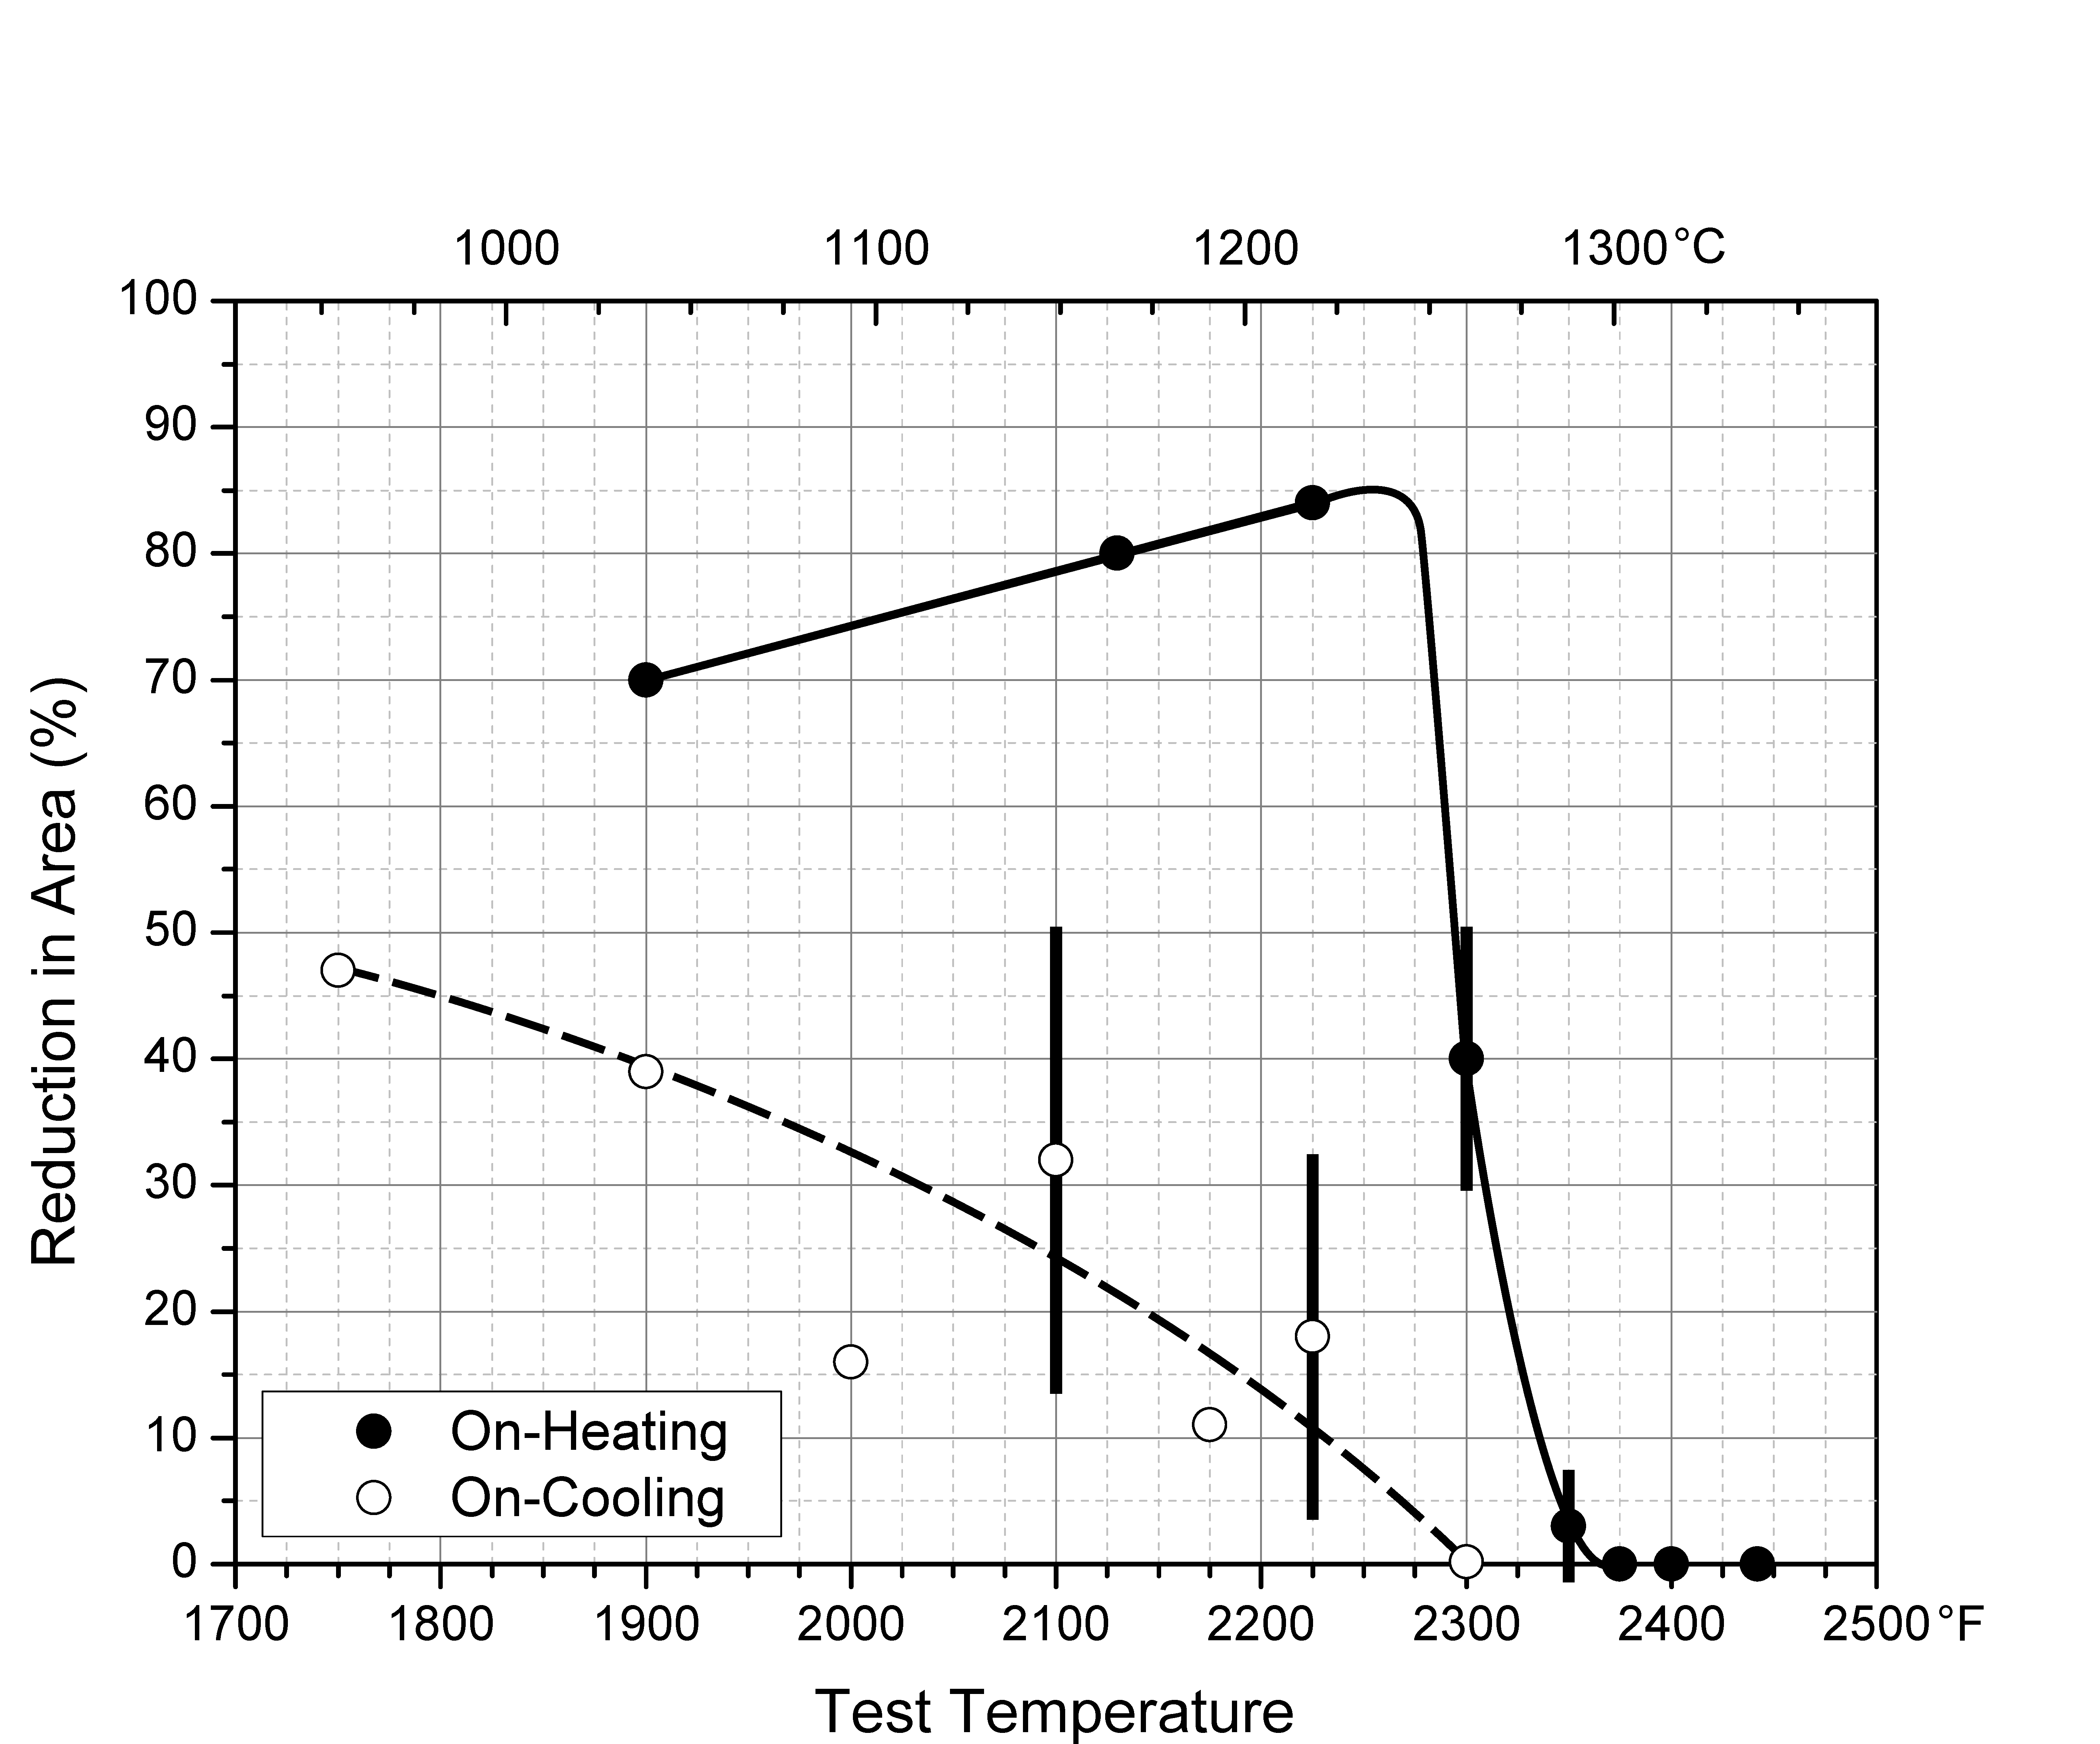
\includegraphics[width=6in]{figures/hot-ductility/c1-hot-ductility-curve.pdf}
\caption[Hot Ductility Behavior of Cone~1 Base Metal.]{Hot Ductility Behavior of CT15C Cone~1 Base Metal.  Bars indicate range of \%RA values at indicated test temperature.  On-Heating Curve Exhibits Class H1 behavior with \gls{zdt} = 2375\textdegree{}F; On-Cooling Curve (from Peak Temperature of 2375\textdegree{}F) Exhibits Class C3 behavior.  \gls{drr}(2225\textdegree{}F) = 21\%. Hot Ductility Test Parameters Given in Table~\ref{tab:hot-ductility-parameters}.}
\label{fig:c1-hot-ductility}
\end{figure}

\begin{figure}[h!]
\setlength{\abovecaptionskip}{15pt}
\centering
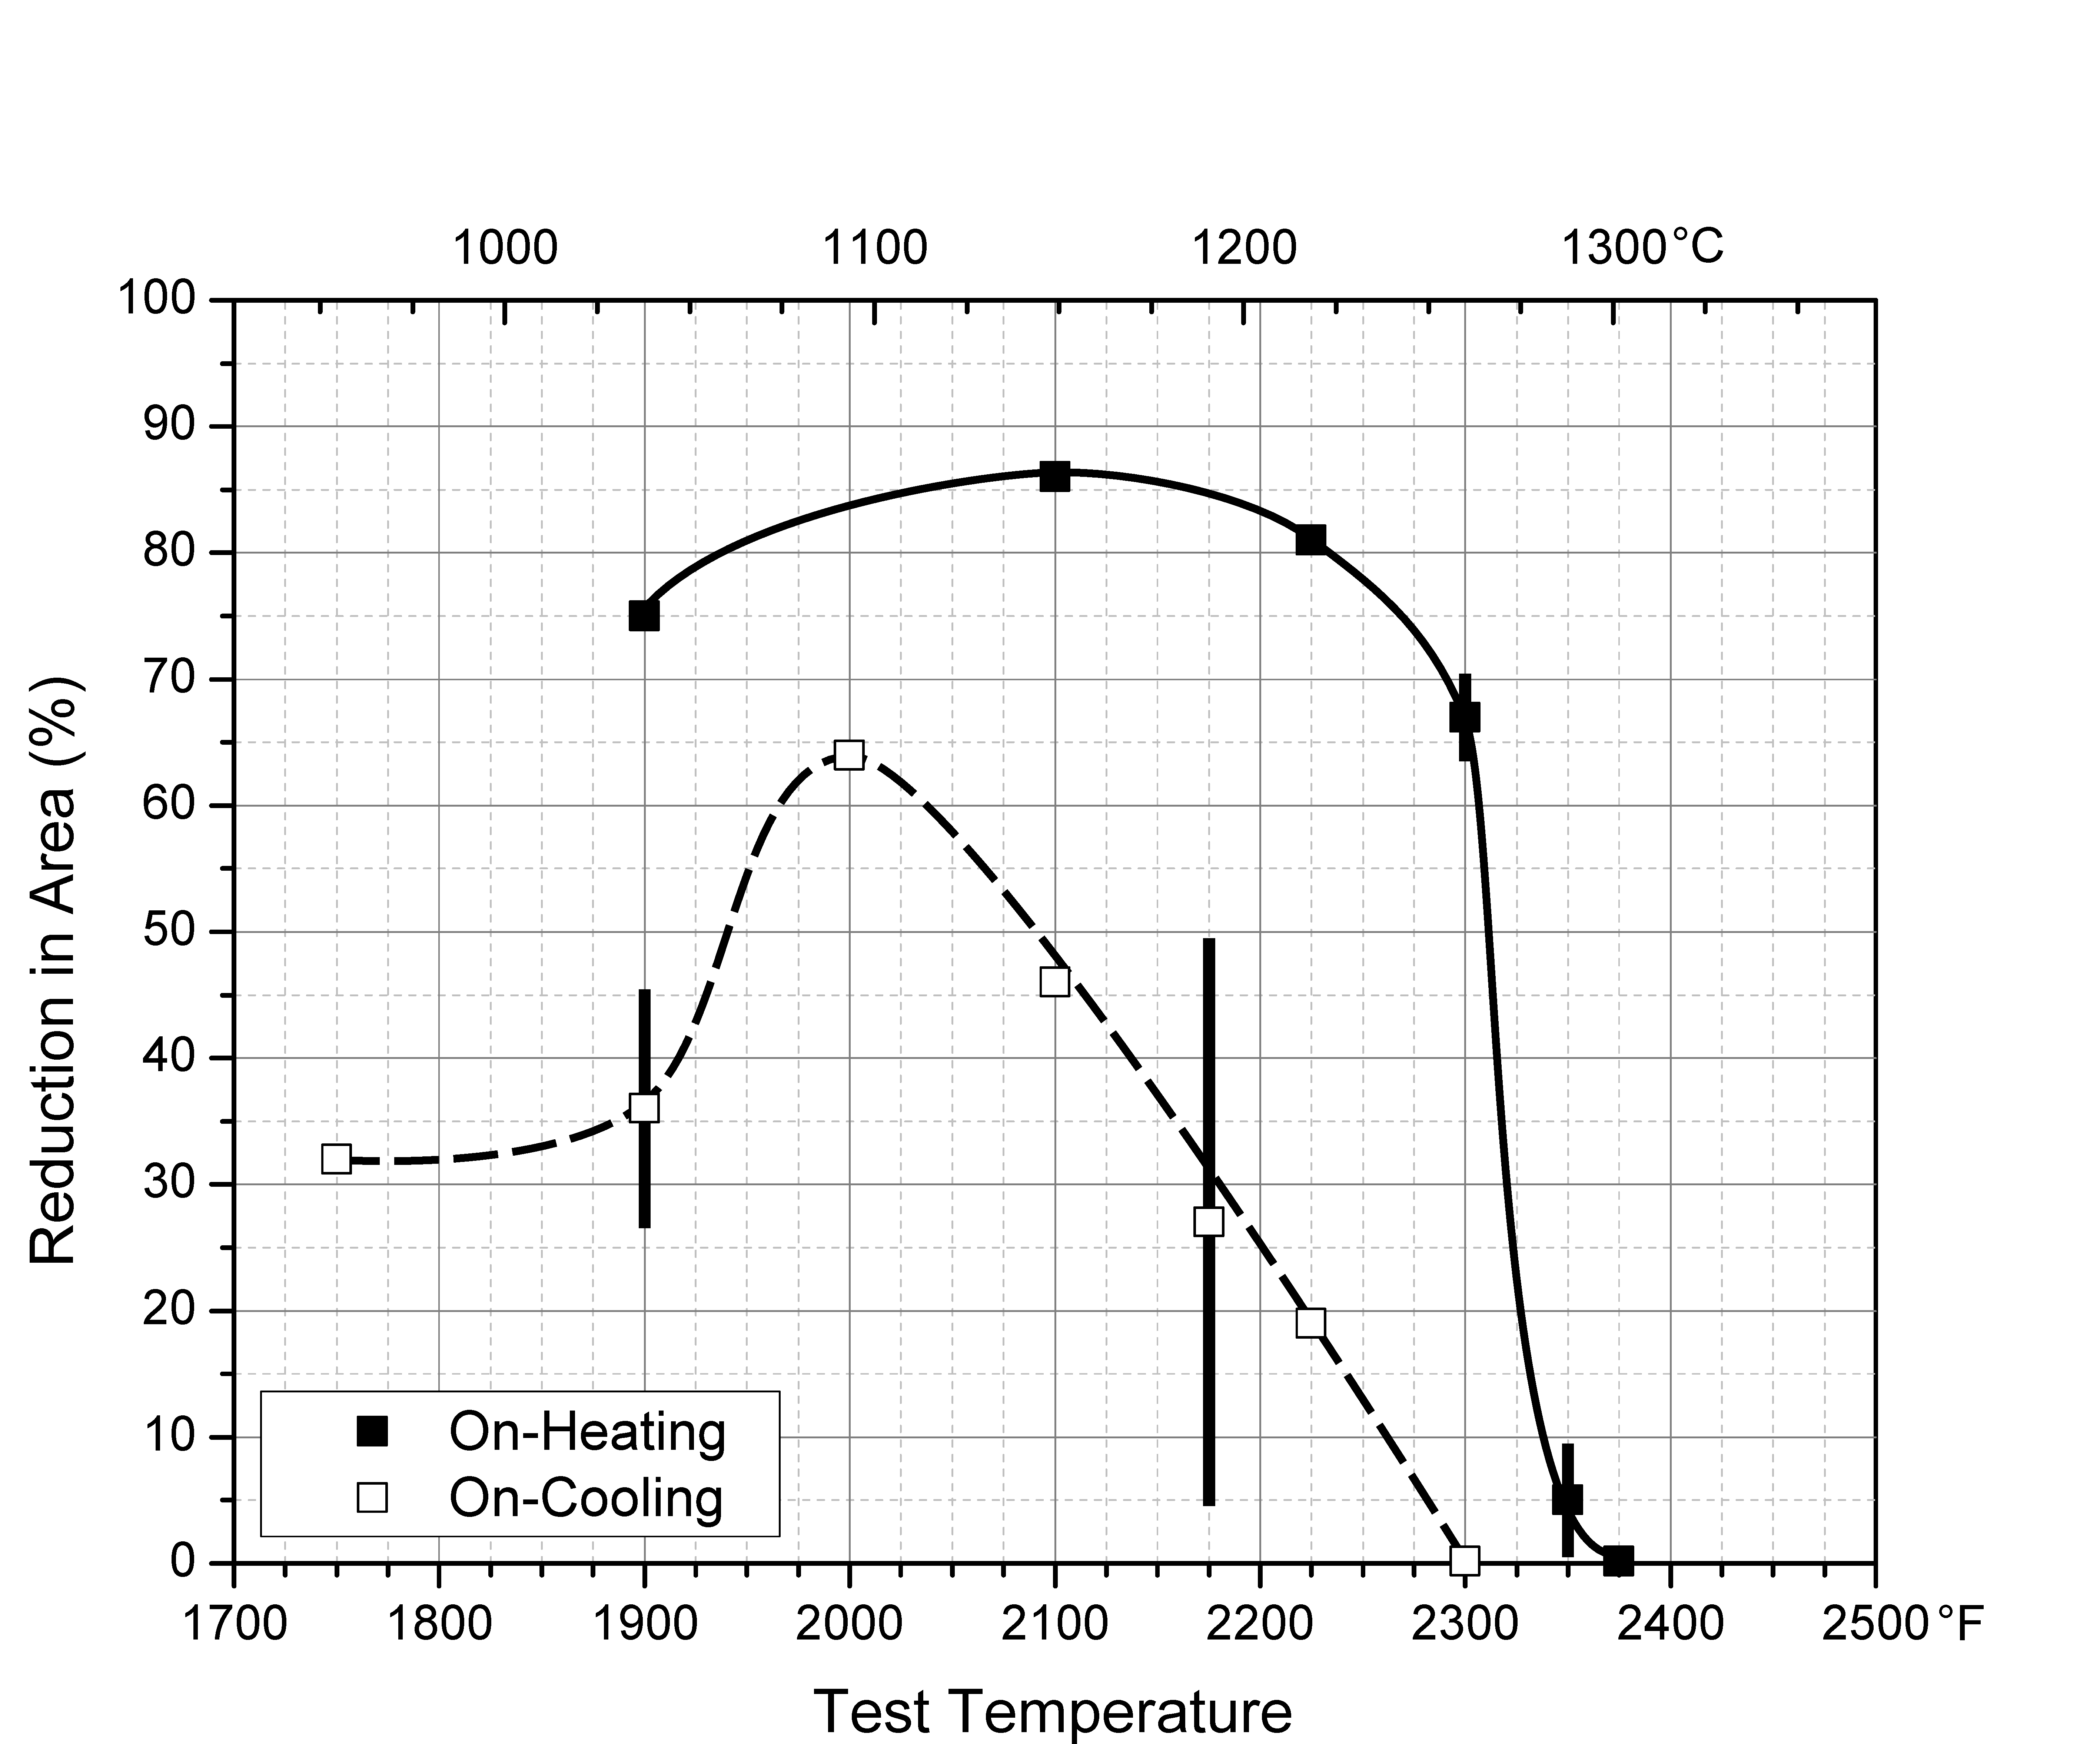
\includegraphics[width=6in]{figures/hot-ductility/c5-hot-ductility-curve.pdf}
\caption[Hot Ductility Behavior of Cone~5 Base Metal.]{Hot Ductility Behavior of CT15C Cone~5 Base Metal.  Bars indicate range of \%RA values at indicated test temperature.  On-Heating Curve Exhibits Class H1 behavior with \gls{zdt} = 2375\textdegree{}F; On-Cooling Curve (from Peak Temperature of 2375\textdegree{}F) Exhibits Class C3 behavior.  \gls{drr}(2225\textdegree{}F) = 23\%. Hot Ductility Test Parameters Given in Table~\ref{tab:hot-ductility-parameters}.}
\label{fig:c5-hot-ductility}
\end{figure}

\begin{table}[h]
\caption{Summary of hot ductility characteristics for Cone~1 and Cone~5 materials, as determined from the curves in Figure~\ref{fig:c1-hot-ductility} and Figure~\ref{fig:c5-hot-ductility}.}
\begin{tabular}{ lccc }
\toprule
\textbf{Material ID and Condition} & \textbf{\gls{zdt} (F)} & \textbf{\gls{drt} (F)} & \textbf{\gls{ndr} (\gls{zdt}-\gls{drt}) (F)} \\
\midrule
Cone~1 (Service-Exposed) & 2375 & 2300 & 75 \\
Cone~5 (Nominally solution-annealed) & 2375 & 2300 & 75 \\
\bottomrule
\end{tabular}
\label{tab:hot-ductility-results}
\end{table}

As can be seen from Figure~\ref{fig:c1-hot-ductility} and Figure~\ref{fig:c5-hot-ductility}, the on-heating hot ductility curves for both Cone materials appear similar, with similar reduction in area (\% RA) values at each test temperature, except in the vicinity of 2300\textdegree{}F.  At this temperature, Cone~1 exhibits a more rapid loss in ductility than Cone~5.  Based on the Nippes evaluation criteria \cite{nippes_further_1957} described previously, examination of the shape of the on-heating ductility curves in Figure~\ref{fig:c1-hot-ductility} and Figure~\ref{fig:c5-hot-ductility} shows that both Cones exhibit Class H1 on-heating hot ductility behavior rather than Class H2 behavior.  This observation regarding the Cone~1 and Cone~5 materials is indeterminate on its own, as \citet{nippes_further_1957} observed in some cases that two materials which both showed H1 on-heating behavior were later found to exhibit either crack-sensitive or crack-insensitive characteristics when tested on-cooling.

Considering the shapes of the on-cooling ductility curves for the Cone~1 and Cone~5 materials after exposure to a peak temperature corresponding to the on-heating \gls{zdt} (2375\textdegree{}F) as shown Figure~\ref{fig:c1-hot-ductility} and Figure~\ref{fig:c5-hot-ductility}, it is apparent that both Cone materials exhibit Class C3 on-cooling behavior when exposed to the \gls{zdt}, based on the Nippes criteria (Figure~\ref{fig:nippes-criteria}).  This category of on-cooling behavior is associated with the greatest degree of hot cracking susceptibility as established by \citet{nippes_further_1957}.  While in general both materials exhibit Class C3 behavior, it appears from Figure~\ref{fig:c1-hot-ductility} and Figure~\ref{fig:c5-hot-ductility} that Cone~5 shows a slightly better qualitative recovery of on-cooling ductility than Cone~1.  As shown in Figure~\ref{fig:c5-hot-ductility}, the on-cooling ductility for Cone~5 recovers to higher values than for Cone~1, particularly at 2100\textdegree{}F and 2000\textdegree{}F.  However, when considering the apparent difference, it should be noted that both Cones are cast components with a large dendrite size, and it was observed in early work on hot ductility by \citet{nippes_further_1957} that castings typically showed wider variation in ductility values at a given test temperature than was observed for wrought material.  The 20Cr-32Ni-1Nb cast material used in both Cones is no different in this regard, for example as evidenced by the variation at 2100\textdegree{}F on-cooling for Cone~1 and 2175\textdegree{}F on-cooling for Cone~5.  Due to the reality of variations in ductility values, it is recommended practice (\citet{lundin_standardization_1990_experiment}) to run a minimum of two hot ductility tests at each temperature, with some studies (\citet{nippes_further_1957}) running up to four tests per temperature for cast materials.  Unfortunately, the number of samples available in the current study was not sufficient to permit duplicate tests at all test temperatures; however, duplicates were performed wherever possible, including at the \gls{zdt}.  If sufficient samples had been available for duplicate tests at all temperatures, it is possible that the average \% RA at certain test temperatures (e.g. 2000\textdegree{}F on-cooling and 2100\textdegree{}F on-cooling) would be closer in magnitude between Cone~1 and Cone~5.  Taking these considerations into account, it is likely that Cone~1 and Cone~5 are more similar in on-cooling behavior than would be suggested by a casual inspection of the curves in Figure~\ref{fig:c1-hot-ductility} and Figure~\ref{fig:c5-hot-ductility}.

To quantify the severity of the on-cooling ductility loss exhibited by both materials, the ductility recovery rate (\gls{drr}) was determined for both Cone~1 (Figure~\ref{fig:c1-hot-ductility}) and Cone~5 (Figure~\ref{fig:c5-hot-ductility}) at a test temperature of 2225\textdegree{}F since this corresponds most closely with the observed rapid-ductility-decrease temperature (on-heating) for both Cones.  The \gls{drr} at 2225\textdegree{}F was similarly low for both Cone materials: 21\% for Cone~1 and 23\% for Cone~5.  Additionally, both Cones exhibited a region of zero on-cooling ductility (a \gls{zdr}) after exposure to the on-heating \gls{zdt}; for both Cone~1 and Cone~5, the \gls{zdr} is 75F\textdegree{} wide (2300–2375\textdegree{}F).  Considered together, the occurrence of Class C3 cooling behavior, the relatively low \gls{drr} values, and the presence of a significant \gls{zdr} all indicate that the Cone~1 and Cone~5 materials are both susceptible to liquation cracking when exposed to temperatures typically experienced during a welding thermal cycle. Compared to other heat-resistant alloys, the hot ductility behavior of 20Cr-32Ni-Nb as revealed in Figures~\ref{fig:c1-hot-ductility} and \ref{fig:c5-hot-ductility} is similar to the behavior of ``cracking sensitive'' heats of Alloy 800H as investigated by Qiao (cite Qiao PhD), for example as shown in Figure ??. Also in Qiao's study, in comparison, heats of 800H categorized as ``cracking insensitive'' showed a much higher \gls{drr} and a minimal \gls{zdr}, and exhibited Class C1 on-cooling behavior, for example as shown in Figure ??.


\section{Microstructural Characterization}
\subsection{As-Received Base Metal Microstructures}
The typical as-received microstructures for the Cone~1 and Cone~5 materials, respectively, are shown in the optical micrographs in Figure~\ref{fig:c1-asreceived} and Figure~\ref{fig:c5-asreceived}.  Both Cone materials exhibited a cast, dendritic structure with a large dendrite size.  The 500X magnification micrographs in Figure~\ref{subfig:c1-asreceived-500X} and Figure~\ref{subfig:c5-asreceived-500X} show the presence of a abundant fine intradendritic precipitates in the austenite matrix in addition to the larger phases along the interdendritic boundaries. The as-received Cone~1 and Cone~5 base metals were also examined in the \gls{sem} to perform \gls{eds} analyses on some of the constituents. \Gls{sem} micrographs and \gls{eds} results for typical Cone~1 and Cone~5 microstructures are presented in Figures \ref{fig:c1-ar-sem} and Y and Figures \ref{fig:c5-ar-sem} and YY, respectively. For Cone~1 material, Figure~\ref{fig:c1-ar-sem }shows both coarse interdendritic phases (e.g. ``A'' in Figure~\ref{subfig:c1-ar-sem-5kx}) and clusters of finer precipitates (``B'' in Figure~\ref{subfig:c1-ar-sem-5kx}). The \gls{eds} results in Figure Y, corresponding to points ``A'' and ``B'' in Figure~\ref{subfig:c1-ar-sem-5kx}, show a high amount of niobium indicating that both regions are niobium carbides (NbC). The chromium, iron, and nickel contents reported for point ``B'' are considered to arise from beam interaction with the surrounding matrix, due to the small size of the analyzed particles. Similarly for the Cone~5 material, Figure~\ref{fig:c5-ar-sem} shows coarse interdendritic phases (``A'' in Figure~\ref{subfig:c5-ar-sem-5kx}) with finer phases present at the periphery (area ``B'' in Figure~\ref{subfig:c5-ar-sem-5kx}). Both ``A'' and ``B'' in Figure~\ref{subfig:c5-ar-sem-5kx} contain a high amount of niobium as shown in Figure YY, corresponding to NbC. The compositions of the very fine (<< \SI{1}{\micro\meter}) intradendritic precipitates, visible in both Cone~1 and Cone~5 in Figure~\ref{subfig:c1-ar-sem-1kx} and Figure~\ref{subfig:c5-ar-sem-1kx} respectively, were not determined because these precipitates are too small to be analyzed with \gls{eds}. 

It should be noted in service-exposed 20Cr-32Ni-Nb material, the NbC carbides are often accompanied by the formation of a secondary phase rich in nickel, niobium, and silicon (``Ni-Nb silicide'') as reported by a number of authors (Shi, Hoffman 2000, Knowles 2004, Patchett 1998). However, the presence of Ni-Nb-Si-rich phases around the NbC carbides was not observed in either the Cone~1 or Cone~5 materials despite the fact they were reported to have ~15 y of service exposure at 1575\textdegree{}F. \citet{hoffman_high_2000-1} observed differences in the extent of Ni-Nb-Si-rich phase formation (which he identified as G-phase) between statically cast tees and centrifugally cast cones with different compositions, with the cone material having a lesser (unspecified) extent of silicide formation. \emph{Compared to the service conditions and materials reported by Shi, Hoffman, Knowles, and Patchett, the material examined in the current study either has a significantly longer service exposure time, higher service temperature, or [lower Si content]. In light of these differences, it is possible that the formation of the Ni-Nb-Si-rich phases is not favored at the service temperatures to which the Cone~1 and Cone~5 materials were subjected. However, the lack of published time-temperature precipitation (TTP) data for the 20Cr-32Ni-Nb alloy (cite Patchet??) makes it difficult to ascertain if this is the case.}

%Ni-Nb-Si phases, cite Shi, Hoffman 2000, KNowles 2004, Patchett 1998, Shibasaki

%Under the beam conditions used for the current analyses, the interaction volume that is sampled by a single ``spot'' \gls{eds} analysis is [volume].

%Figure X and Figure Y present higher magnification SEM micrographs of the typical Cone~1 microstructure along with \gls{eds} results.

\begin{figure}
\centering
\subfloat[100X]{\label{subfig:c1-asreceived-100X}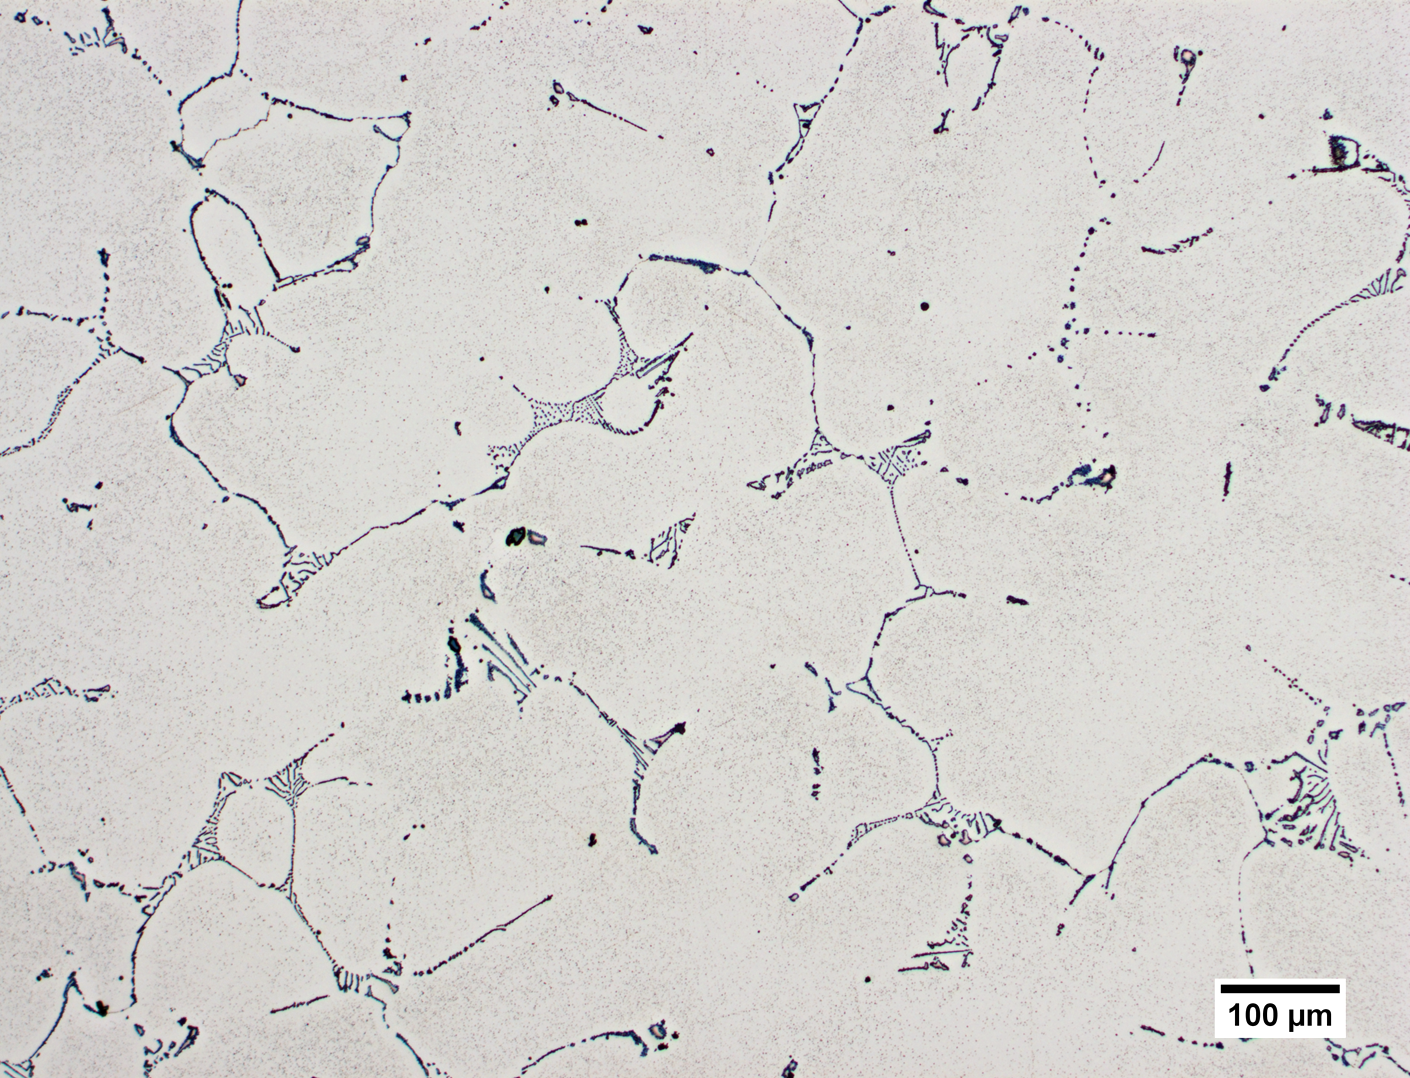
\includegraphics[width=4.7in]{figures/metallography/c1-ar-100X}} \\
\subfloat[500X]{\label{subfig:c1-asreceived-500X}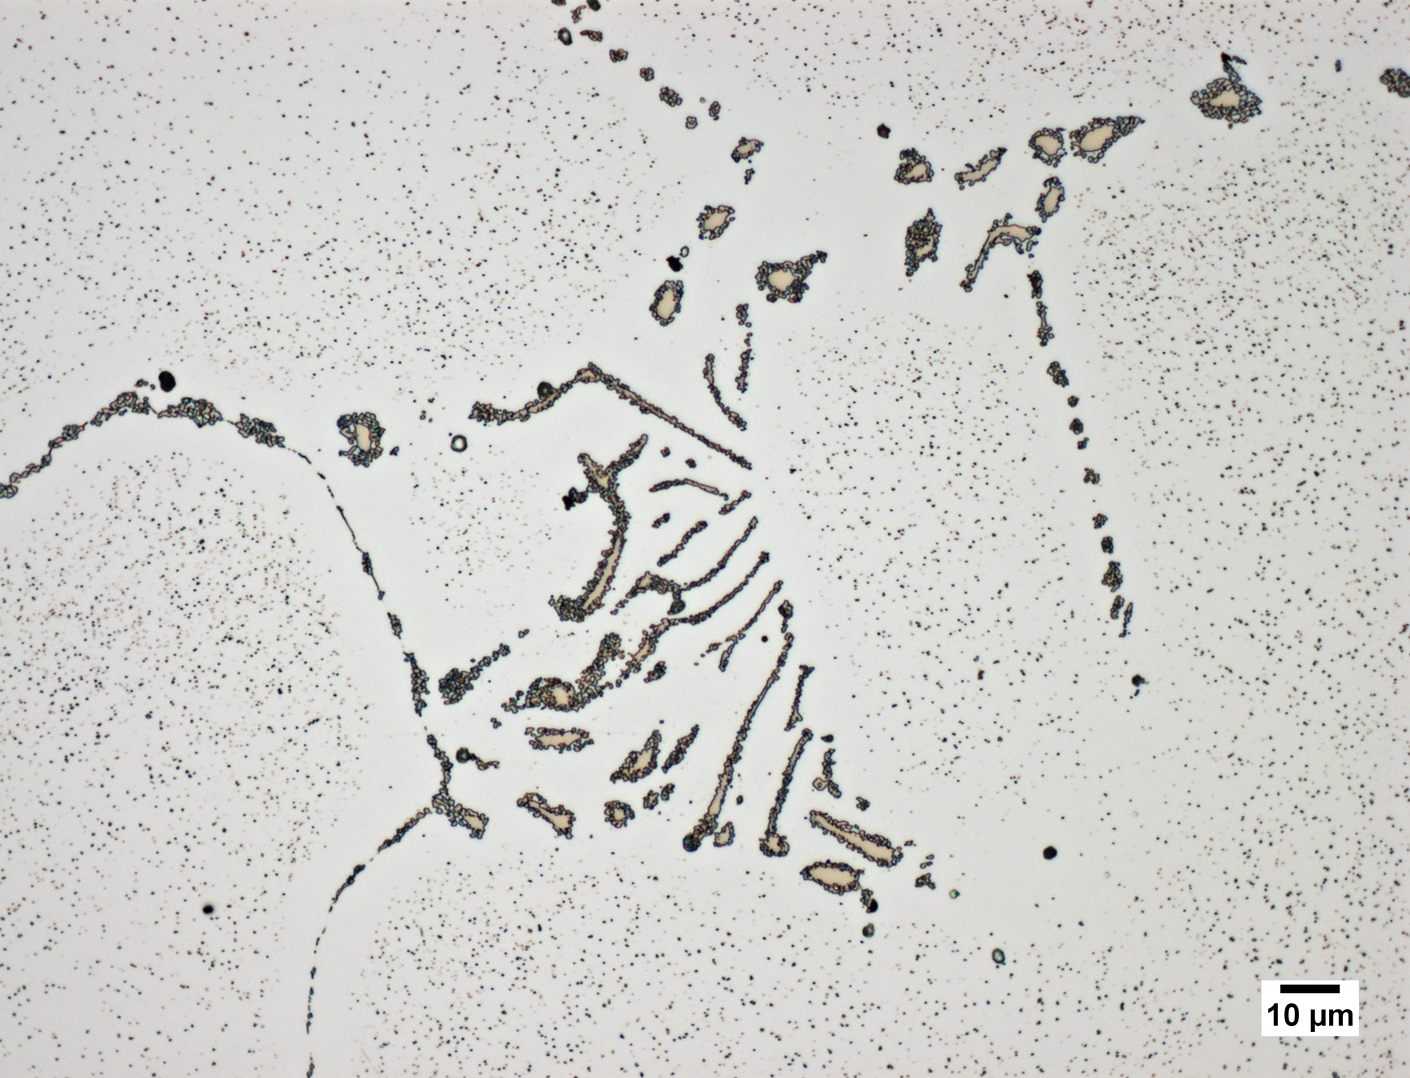
\includegraphics[width=4.7in]{figures/metallography/c1-ar-500X}}
\caption[Optical Micrographs Showing the Typical As-Received Microstructure of Cone~1 Material.]{Optical Micrographs Showing the Typical As-Received Microstructure of Cone~1 Material (Service-Exposed) Utilized for Hot Ductility Testing, (A) 100X and (B) 500X.  Etch: 10\% Oxalic Acid, Electrolytic.}
\label{fig:c1-asreceived}
\end{figure}

\begin{figure}
\centering
\subfloat[100X]{\label{subfig:c5-asreceived-100X}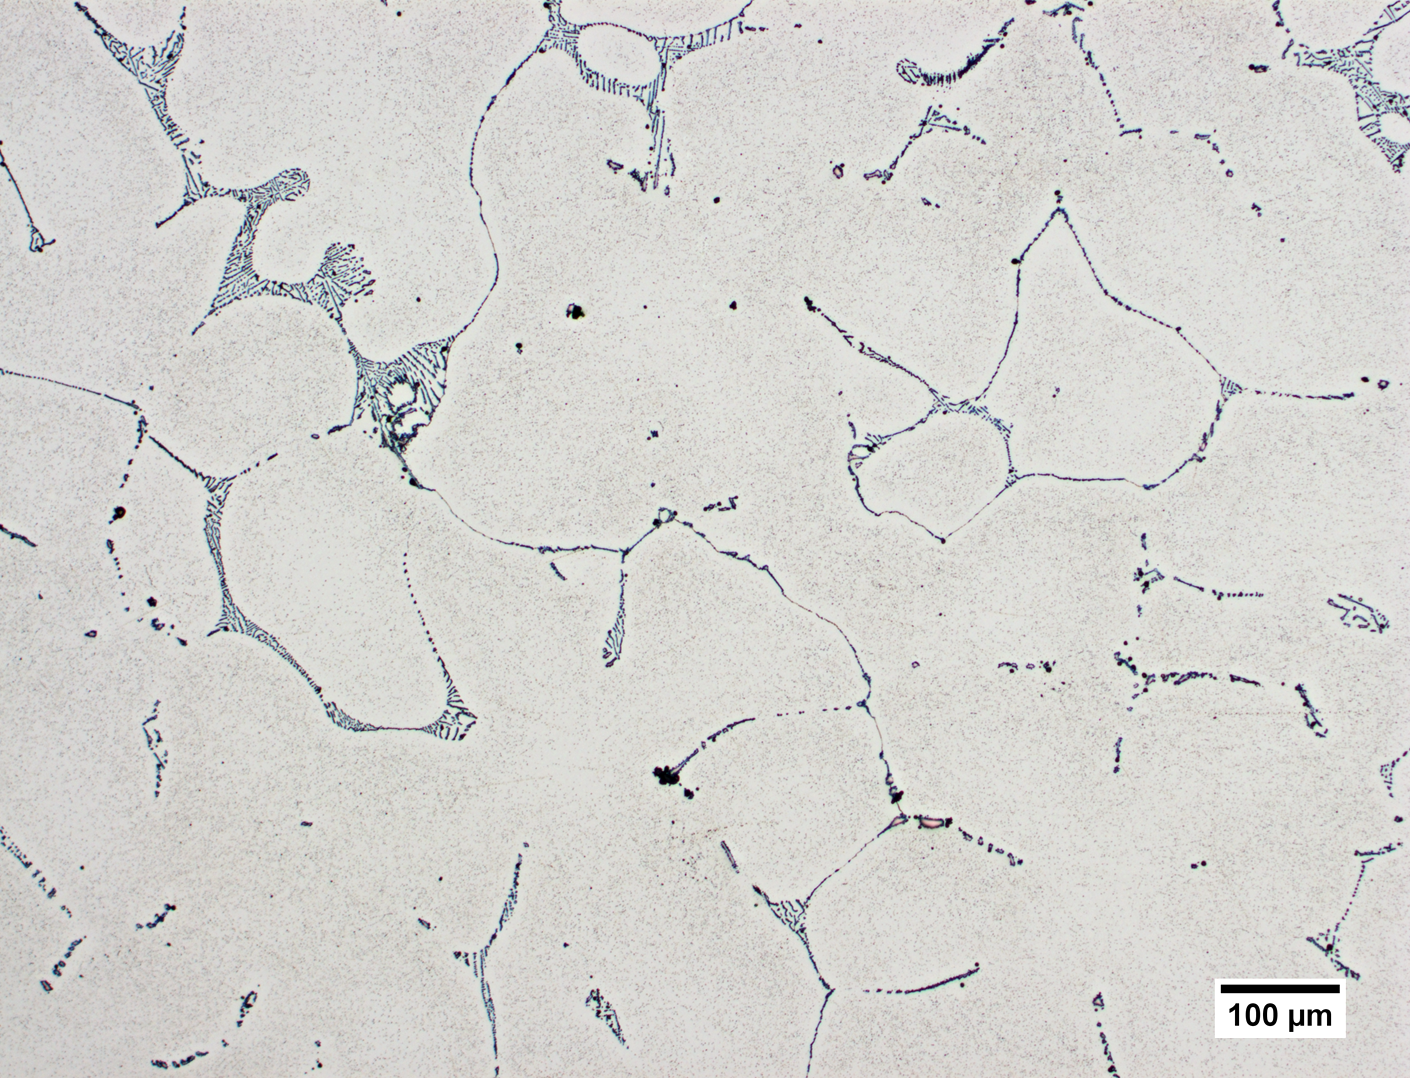
\includegraphics[width=4.7in]{figures/metallography/c5-ar-100X}} \\
\subfloat[500X]{\label{subfig:c5-asreceived-500X}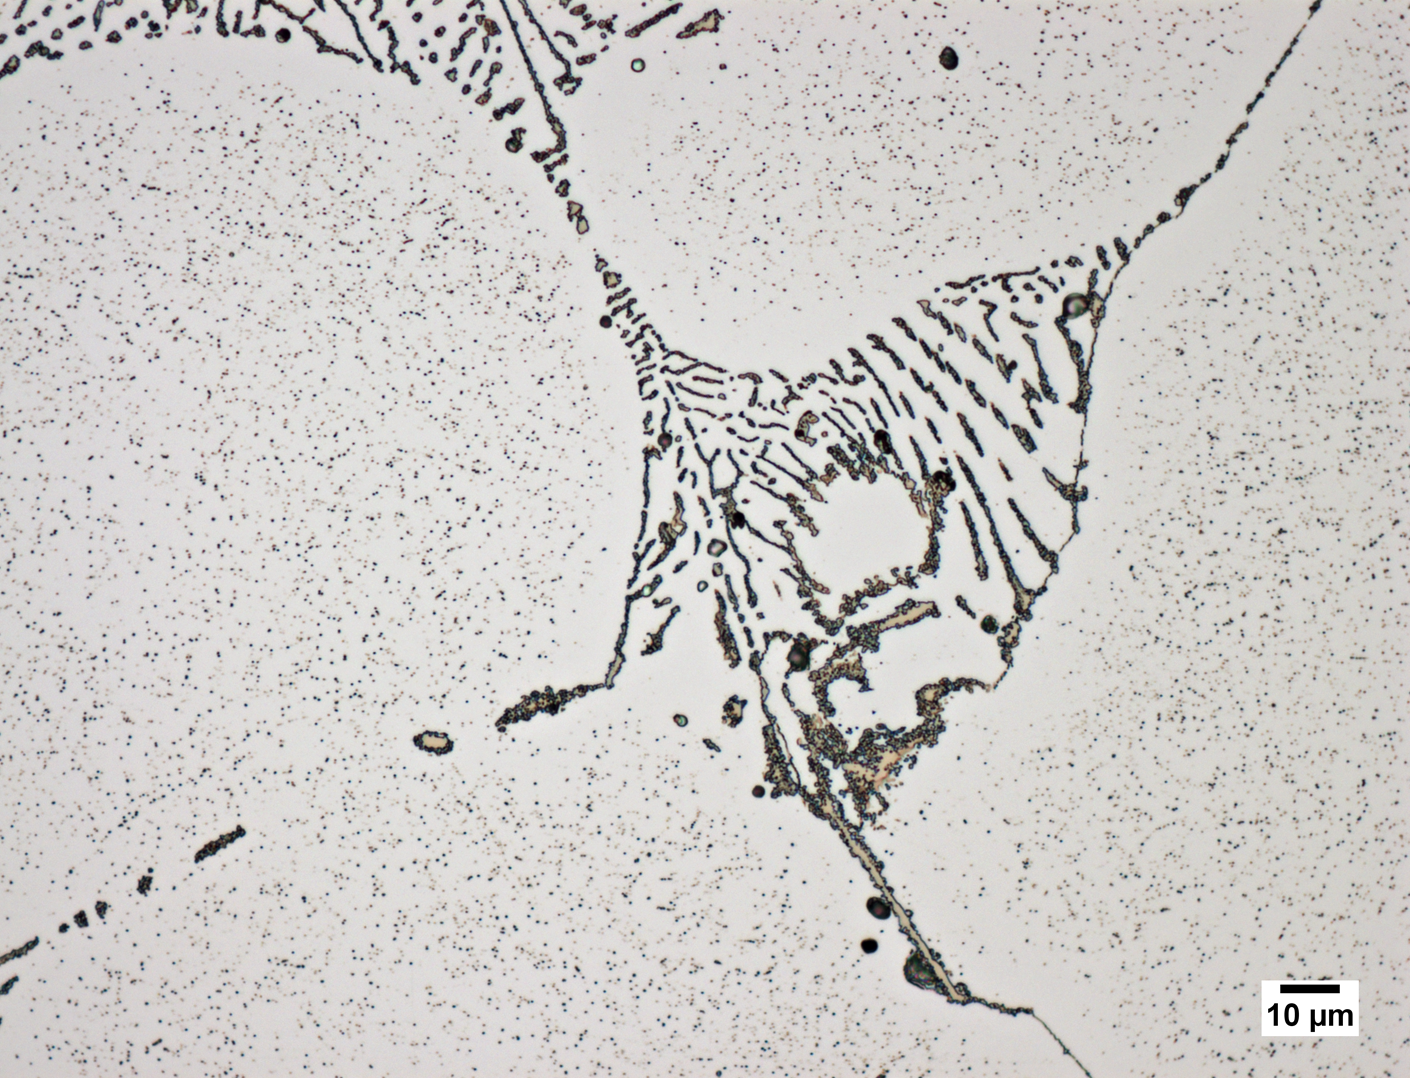
\includegraphics[width=4.7in]{figures/metallography/c5-ar-500X}}
\caption[Optical micrographs showing the typical as-received microstructure of Cone~5 Material.]{Optical micrographs showing the typical as-received microstructure of Cone~5 material (``Solution-Annealed'') utilized for hot ductility testing, (A) 100X and (B) 500X.  Etch: 10\% oxalic acid, electrolytic.}
\label{fig:c5-asreceived}
\end{figure}

%C1 as-received SEM and EDS
\begin{figure}
\centering
\subfloat[1000X]{\label{subfig:c1-ar-sem-1kx}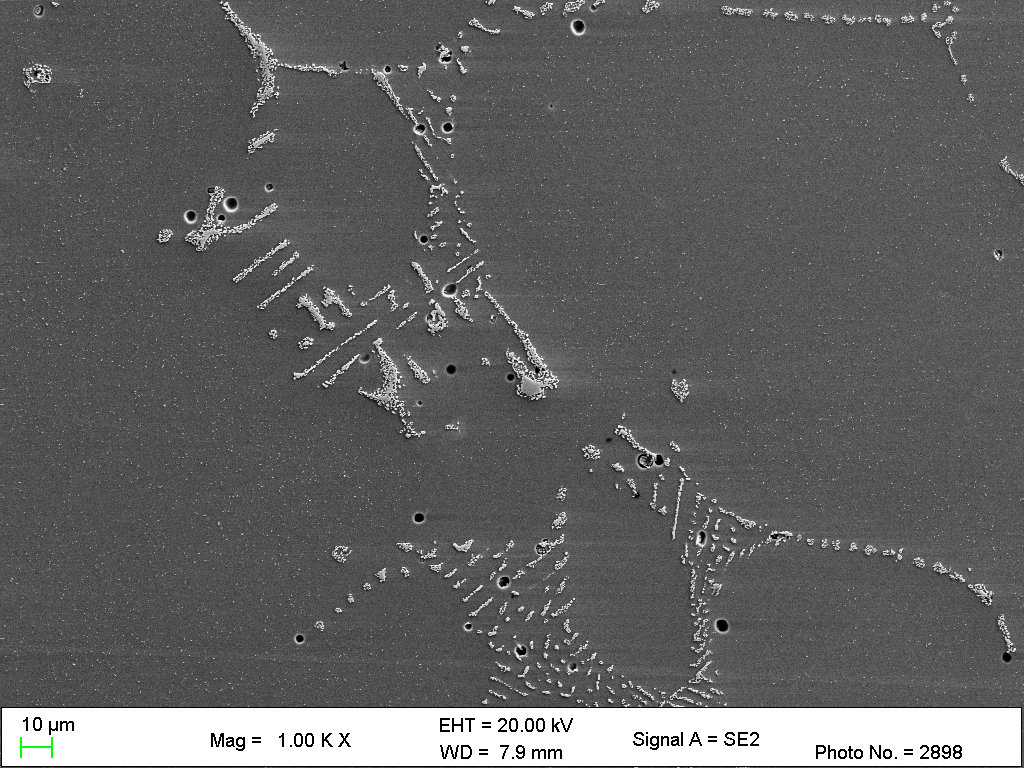
\includegraphics[width=4.7in]{figures/metallography/c1-ar-sem-1kx-L3-08.png}} \\
\subfloat[5000X]{\label{subfig:c1-ar-sem-5kx}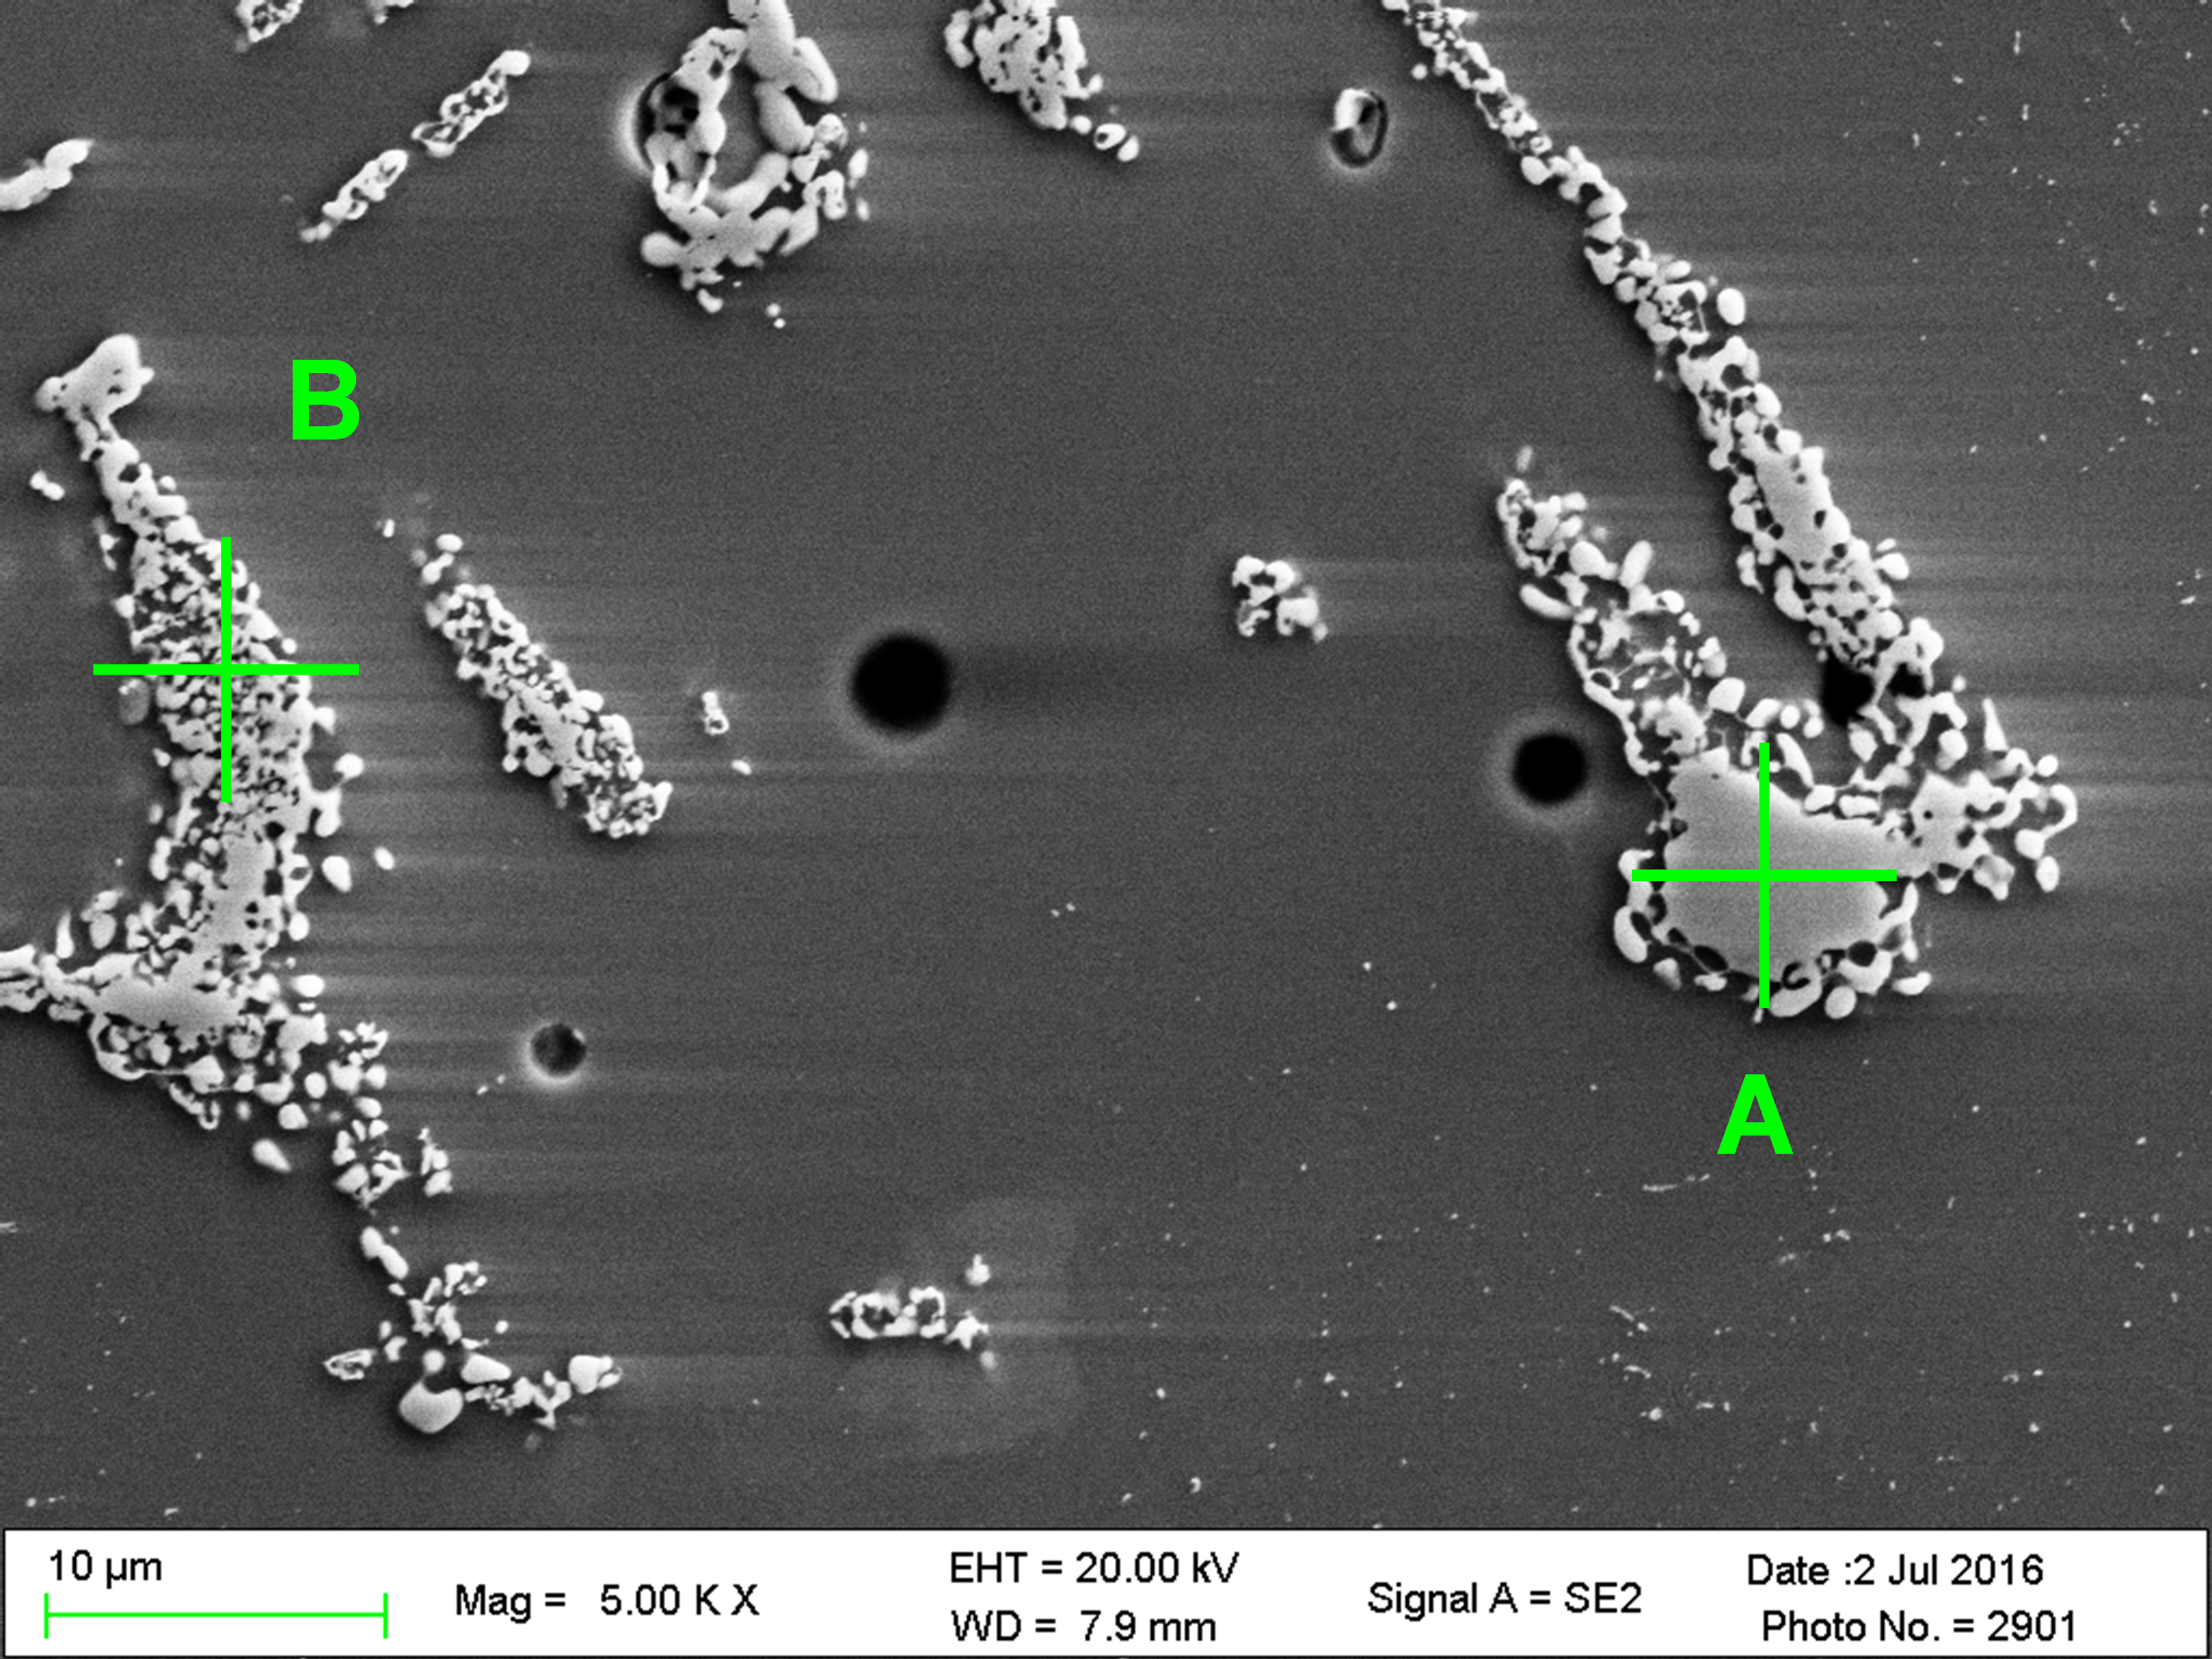
\includegraphics[width=4.7in]{figures/metallography/c1-ar-sem-5kx-L3-11.png}}
\caption[\Gls{sem} micrographs showing typical intradendritic and interdendritic phases present in as-received Cone~1 material.]{\Gls{sem} micrographs showing typical intradendritic and interdendritic phases present in Cone~1 material utilized for hot ductility testing. \Gls{eds} spot analysis results for labeled locations ``A'' and ``B'' are given in Figure~\ref{fig:c1-ar-eds}. Etch: 10\% oxalic acid, electrolytic.}
\label{fig:c1-ar-sem}
\end{figure}

\begin{figure}
\centering
\subfloat[Spot Analysis ``A'']{\label{subfig:c1-ar-eds-a}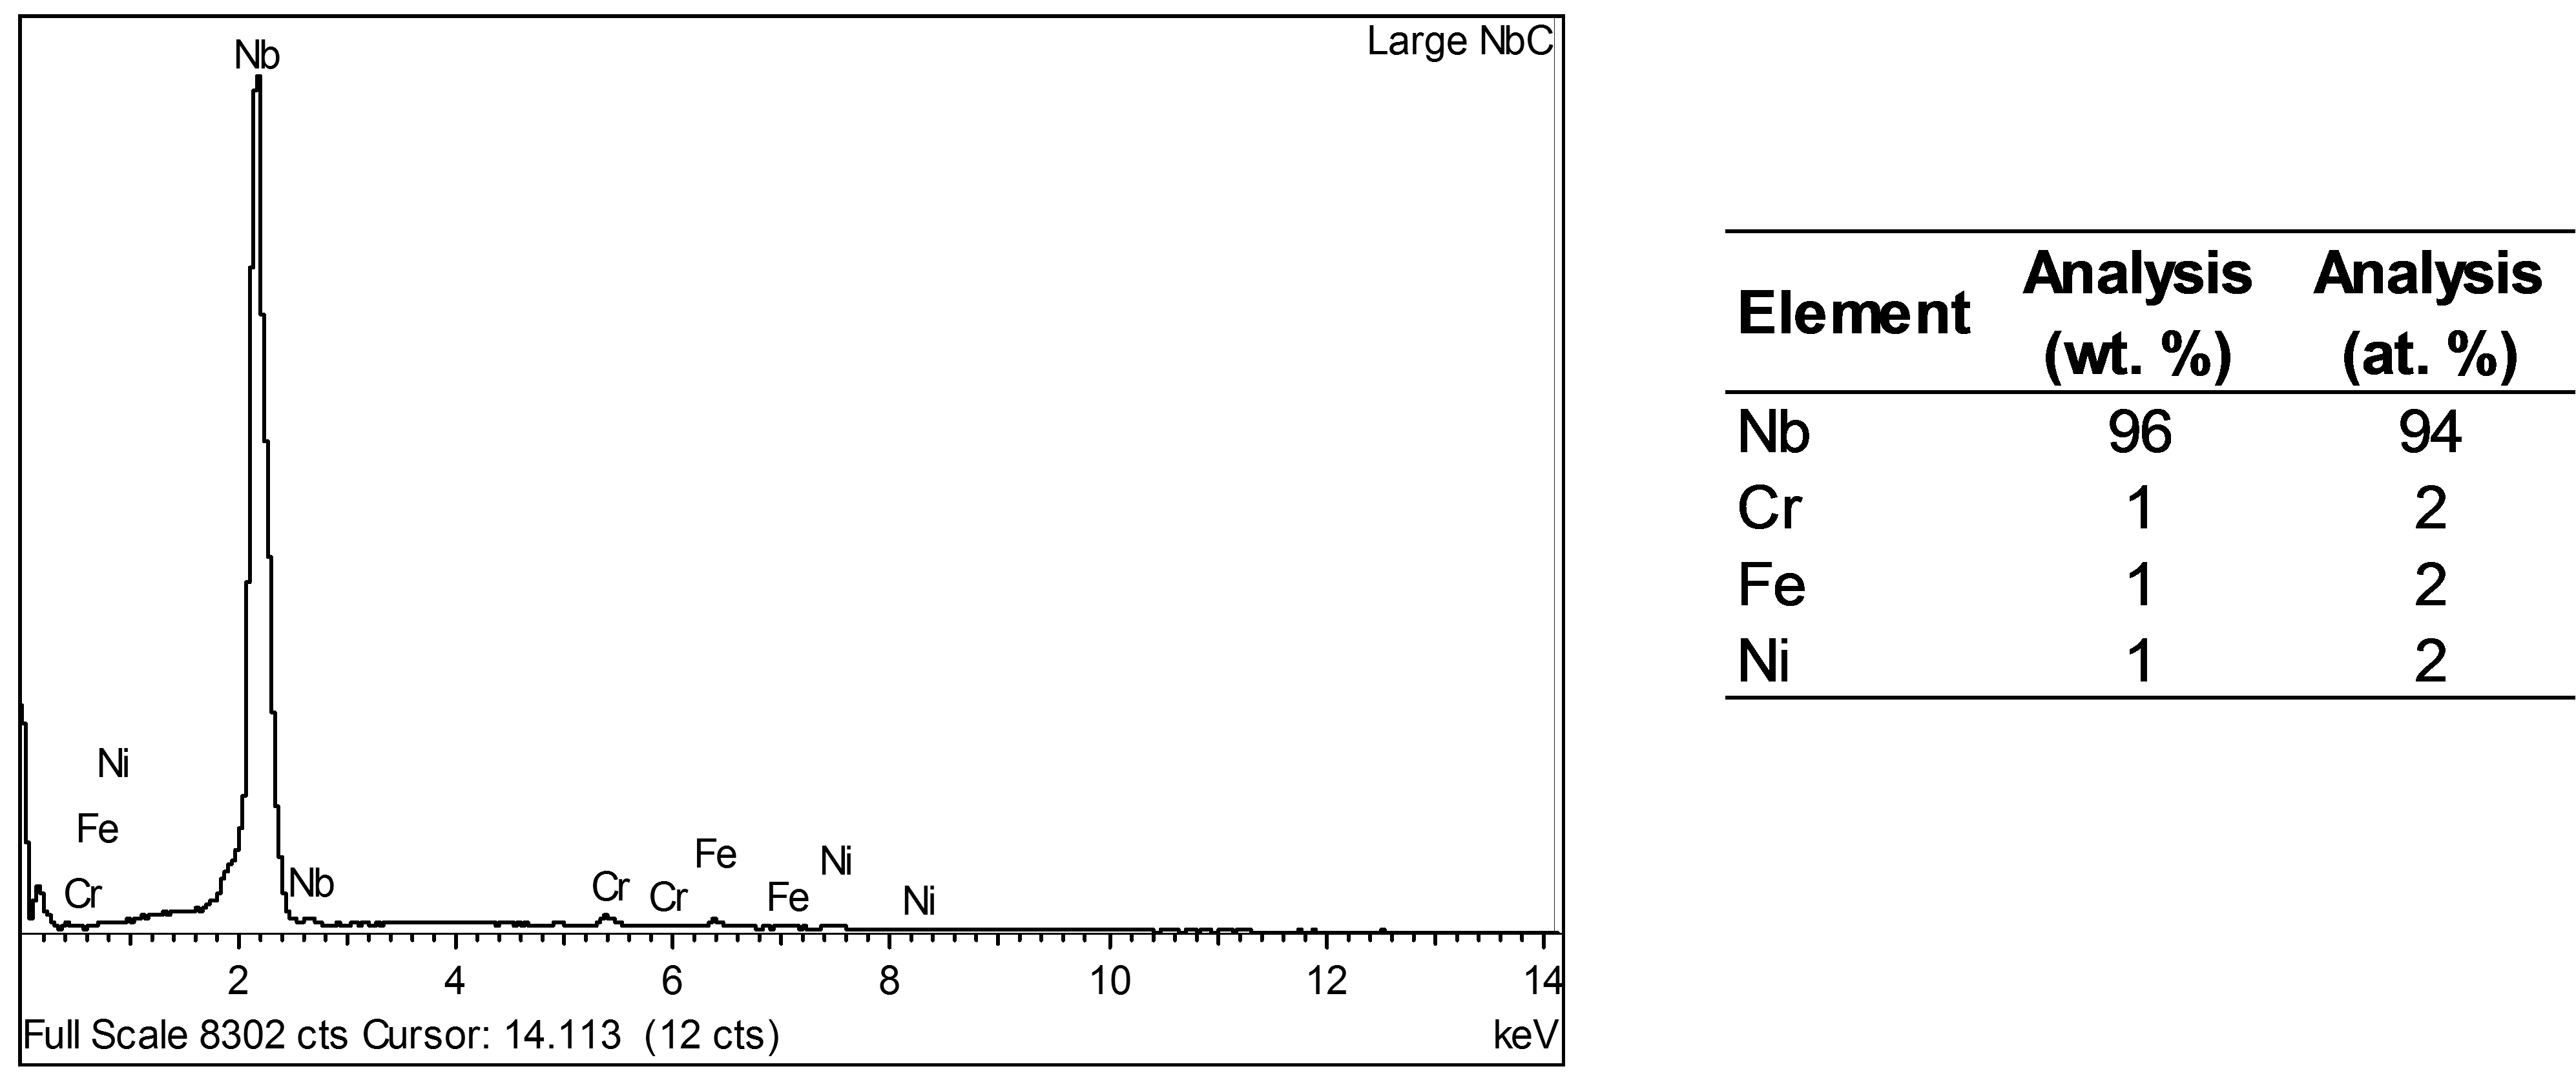
\includegraphics[width=4in]{figures/metallography/c1-ar-eds-table-L3-A.png}} \\
\subfloat[Spot Analysis ``B'']{\label{subfig:c1-ar-eds-b}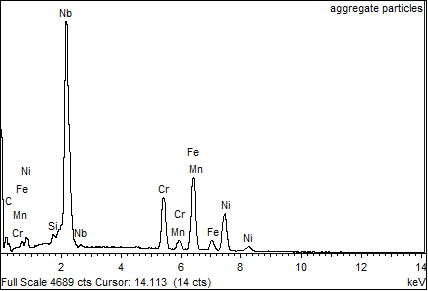
\includegraphics[width=4in]{figures/metallography/c1-ar-eds-L3-B.png}}
\caption[]{\Gls{eds} spot analysis results for locations ``A'' and ``B'' identified in Figure~\ref{subfig:c1-ar-sem-5kx} for as-received Cone~1 material.}
\label{fig:c1-ar-eds}
\end{figure}

%C5 as-received SEM and EDS
\begin{figure}
\centering
\subfloat[1000X]{\label{subfig:c5-ar-sem-1kx}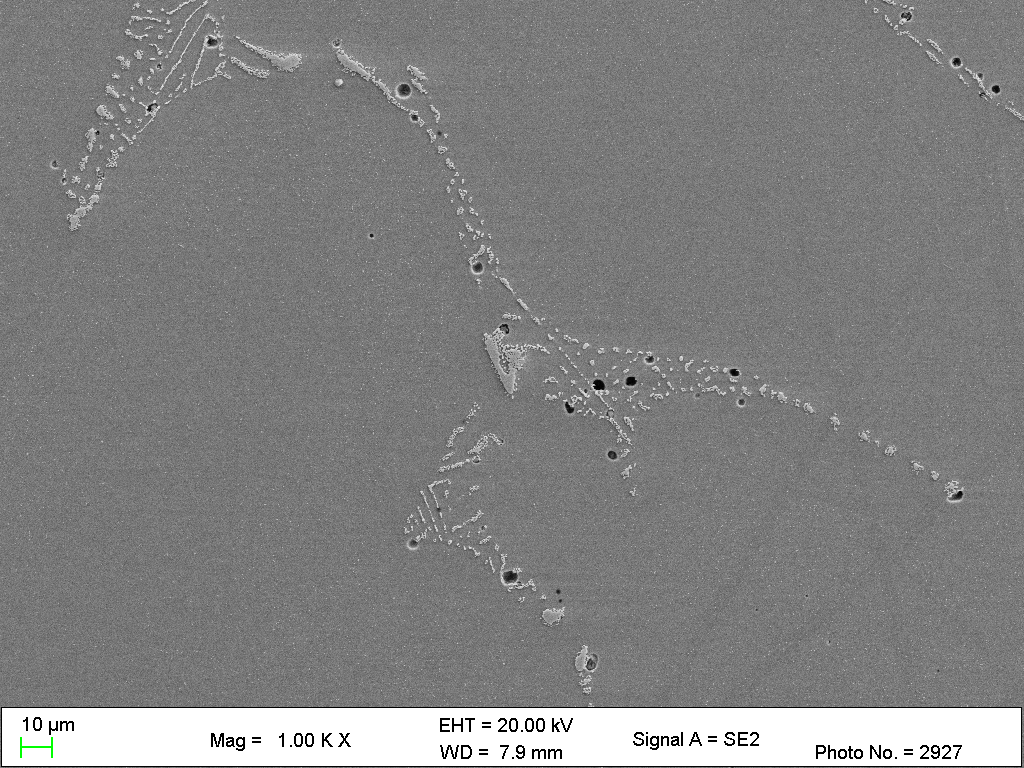
\includegraphics[width=4.7in]{figures/metallography/c5-ar-sem-1kx-L1-10.png}} \\
\subfloat[5000X]{\label{subfig:c5-ar-sem-5kx}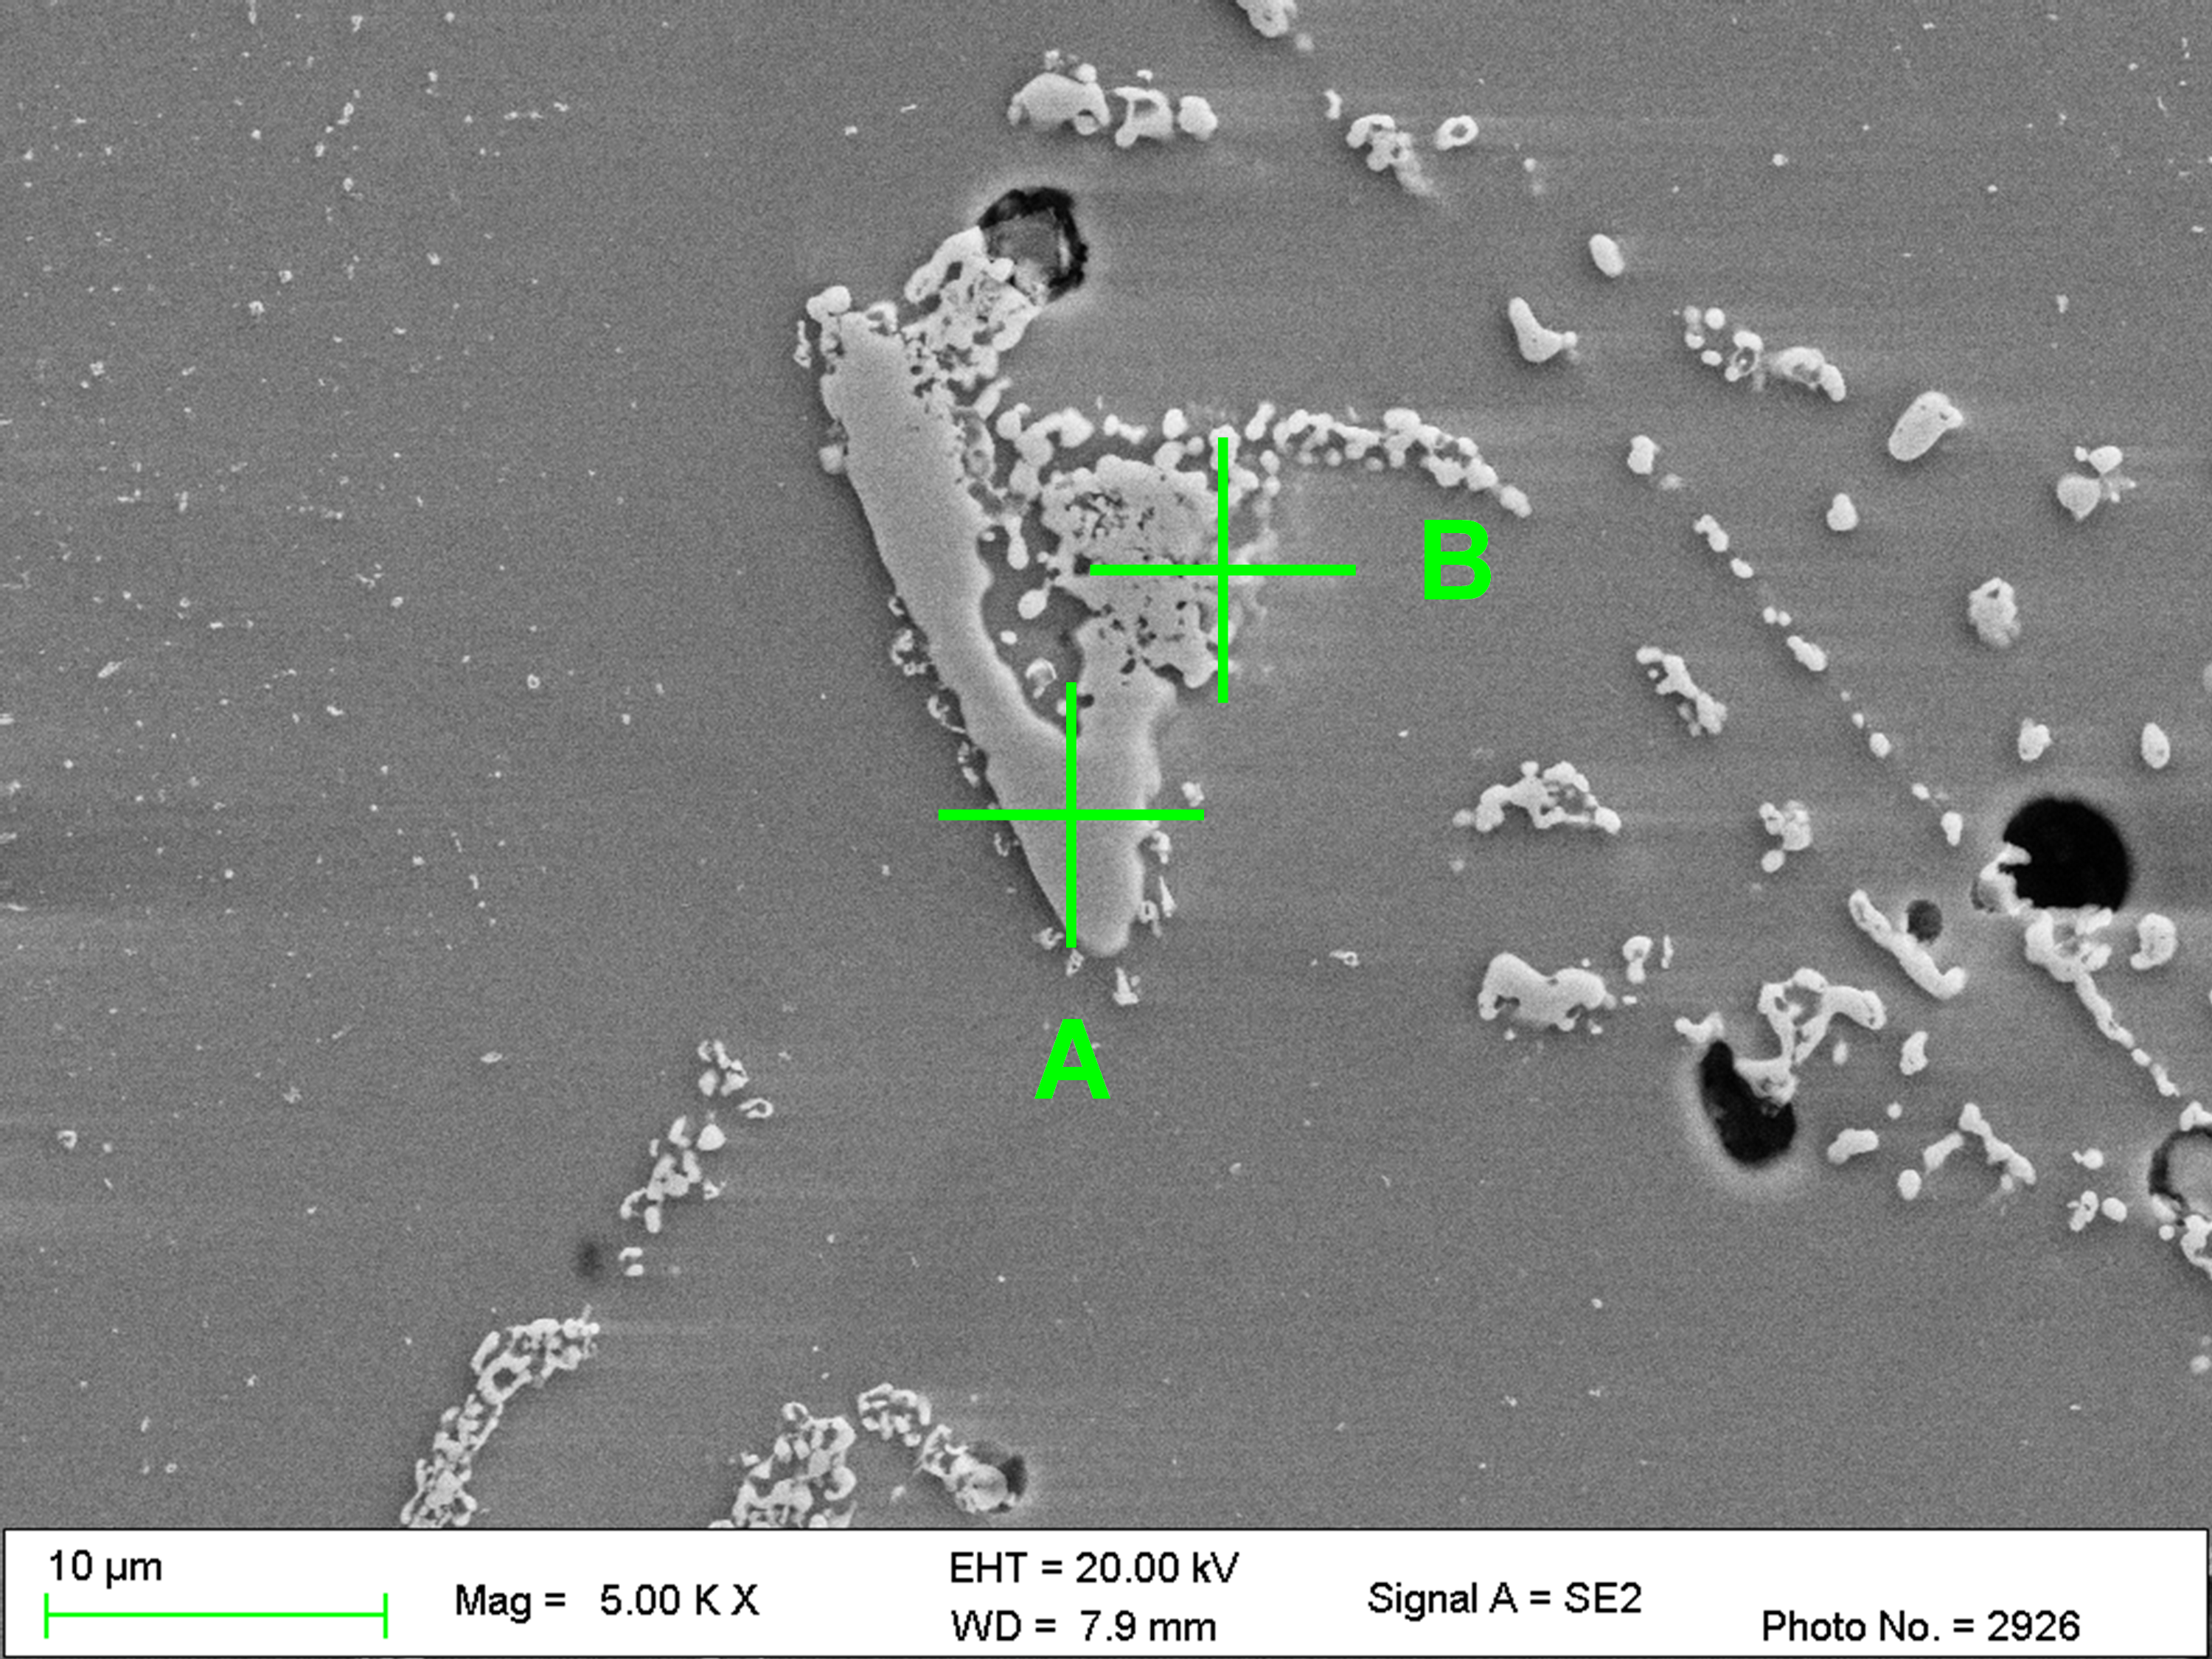
\includegraphics[width=4.7in]{figures/metallography/c5-ar-sem-5kx-L1-09.png}}
\caption[\Gls{sem} micrographs showing typical intradendritic and interdendritic phases present in as-received Cone~5 material.]{\Gls{sem} micrographs showing typical intradendritic and interdendritic phases present in Cone~5 material utilized for hot ductility testing. \Gls{eds} analyses for labeled points ``A'' and ``B'' are given in Figure~\ref{fig:c5-ar-eds}. Etch: 10\% oxalic acid, electrolytic.}
\label{fig:c5-ar-sem}
\end{figure}

\begin{figure}
\centering
\subfloat[Spot Analysis ``A'']{\label{subfig:c5-ar-eds-a}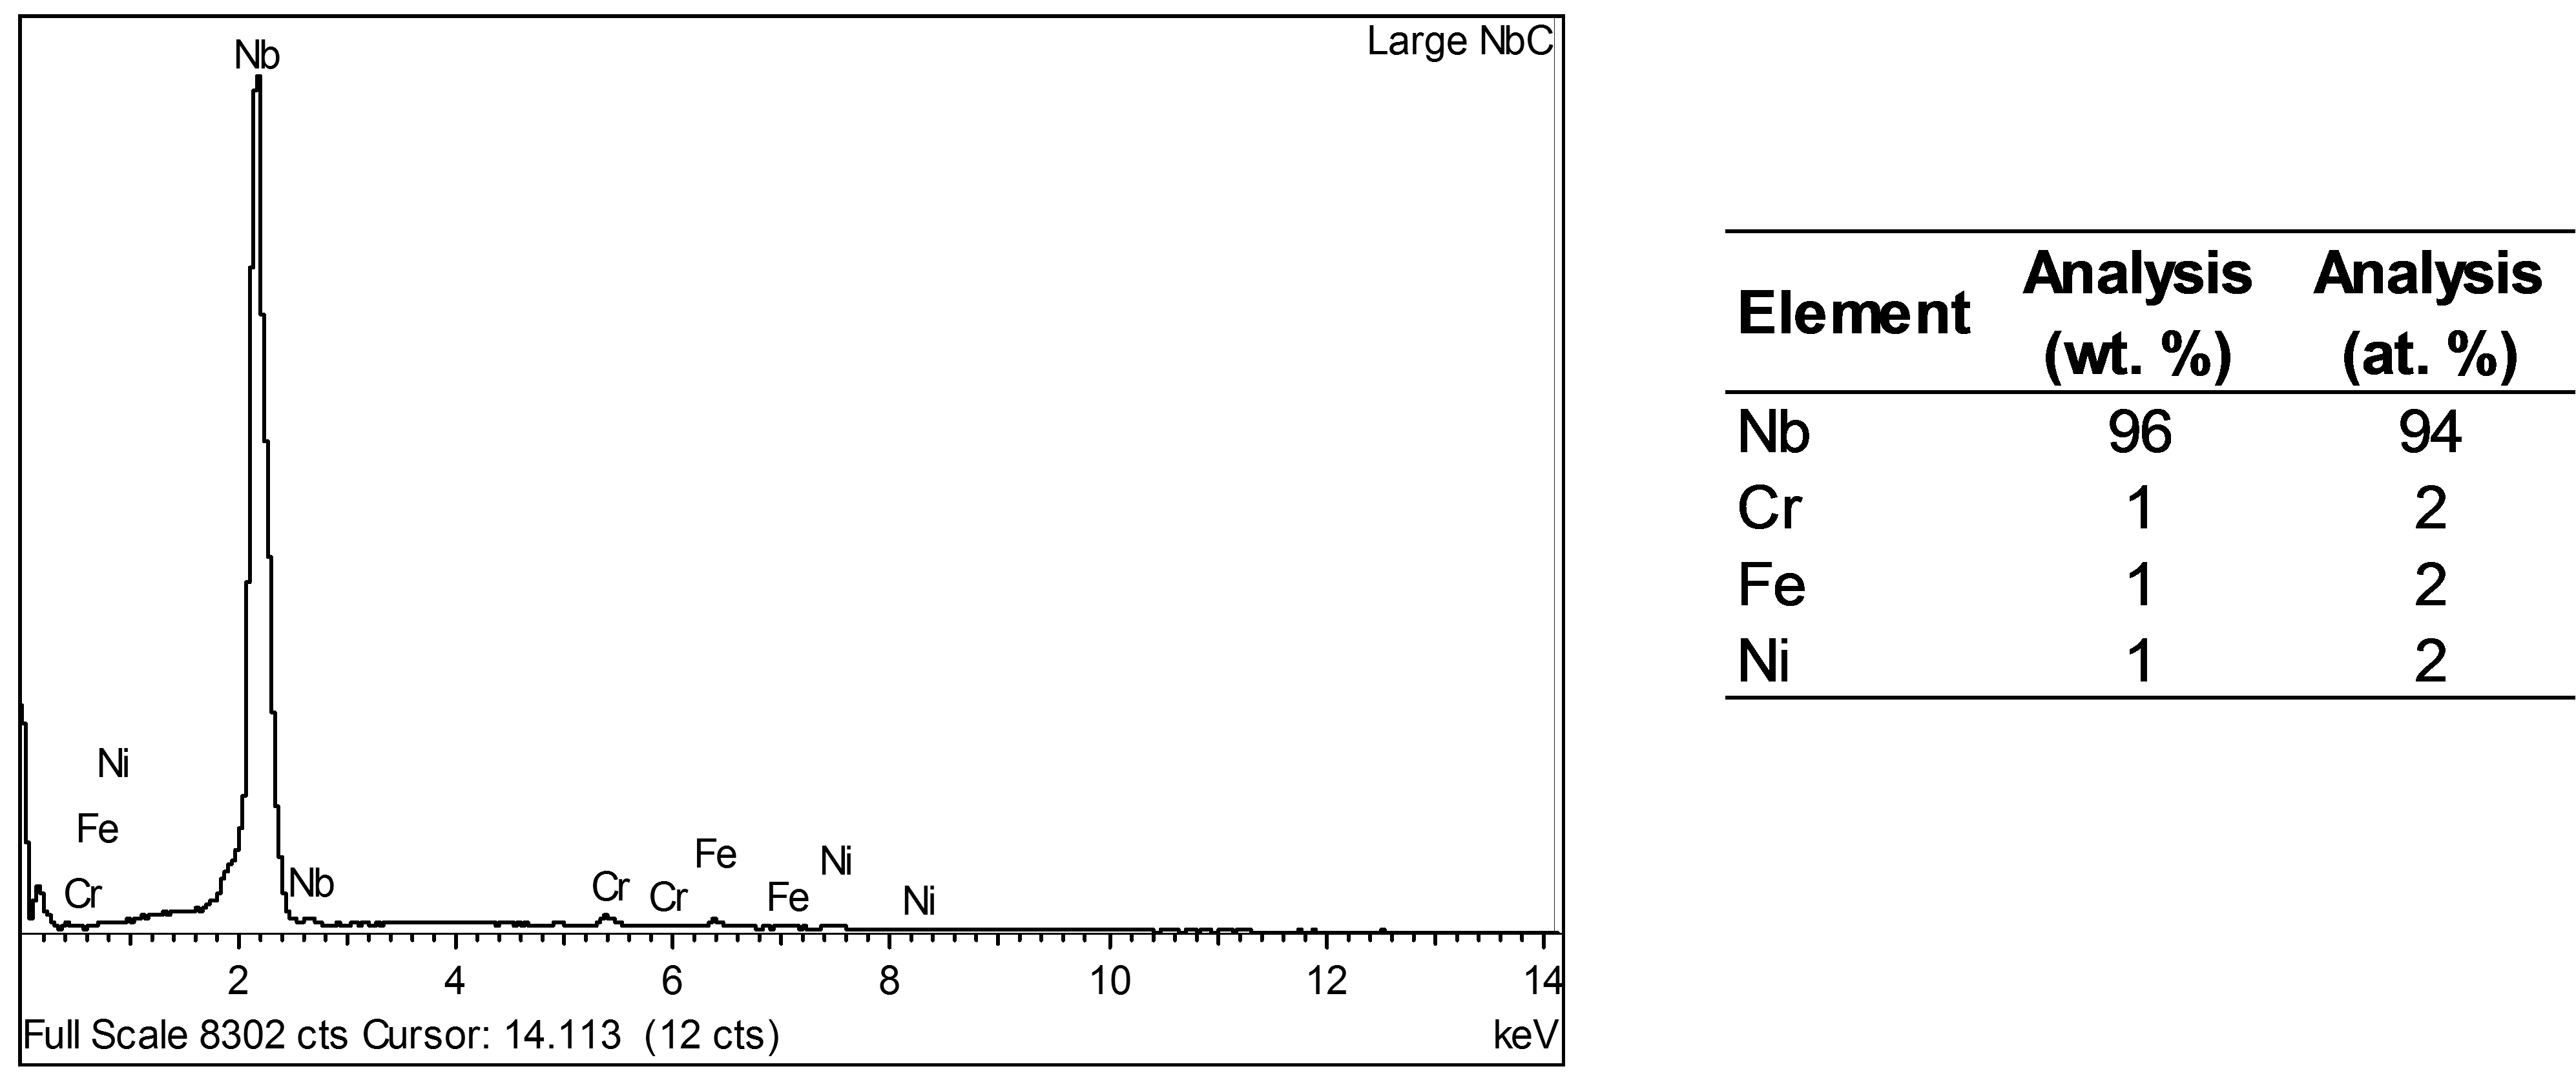
\includegraphics[width=4in]{figures/metallography/c1-ar-eds-table-L3-A.png}} \\
\subfloat[Spot Analysis ``B'']{\label{subfig:c5-ar-eds-b}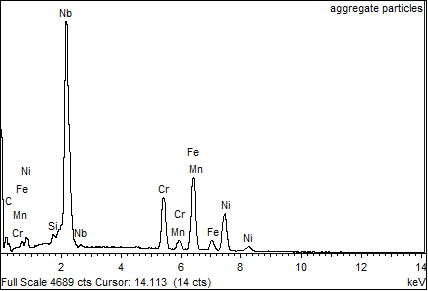
\includegraphics[width=4in]{figures/metallography/c1-ar-eds-L3-B.png}}
\caption[]{\Gls{eds} spot analysis results for locations ``A'' and ``B'' identified in Figure~\ref{subfig:c1-ar-sem-5kx} for as-received Cone~5 material.}
\label{fig:c5-ar-eds}
\end{figure}


\subsection{On-Heating Hot Ductility Tests}
\subsubsection{Cone~1 On-Heating}
Figure X shows a region adjacent to the fracture surface of the Cone~1 On-Heating 2375\textdegree{}F (C1 OH-2375) hot ductility sample. The C1 OH-2375 sample corresponds to the \gls{zdt} for Cone~1 and significant cracking is evident near the surface with the crack paths following the interdendritic boundaries. Note that in Figure X, the tensile loading direction for the hot ductility test is in the vertical direction, so the crack paths are oriented perpendicular to the loading direction. It is also apparent from Figure X, in comparison to the as-received Cone~1 microstructure (Figure~\ref{fig:c1-asreceived}), that dissolution of most of the fine intradendritic precipitates has occurred due to the high temperature of the simulated thermal cycle of the hot ductility test.

The tip of the crack visible in Figure Xa is shown at higher magnification in Figure Xb, which shows evidence of formerly melted regions (where liquid was present) along the crack faces, as well as the interdendritic boundary and associated phases ahead of the crack. The formerly melted regions are denoted by arrows in Figure Xb and are visible as slightly brighter regions which stand faintly in relief. The evidence of liquid along the interdendritic boundaries correlates with the observed zero ductility behavior observed at this temperature. As the peak temperature of the simulated thermal cycle increases to the point where the first liquid (which cannot support strain) is formed along the boundaries, the ductility will drop to zero. Larger formerly-melted regions are also apparent at other locations near the fracture surface in the C1 OH-2375 sample, as shown in Figure Y. However, in general the formerly-melted regions are only intermittently present along the fracture profile (separation surface of the sample) shown in Figure Xa. The melted region from Figure Y is shown at higher magnification in the \gls{sem} micrograph in Figure Z along with spot \gls{eds} results for a location in a formerly-melted region. It is apparent that the formerly-melted region, surrounding the interdendritic phases along a boundary, is not enriched in Ni, Nb, or Si which is in agreement with the results for the as-received Cone 1 base metal which did not find evidence of Ni-Nb-Si-rich phases surrounding the eutectic NbC after service exposure.

%Figures for C1 OH-2375
%Need some EDS of phases
\subsubsection{Cone~5 On-Heating}
Figure A shows a region at the fracture surface of the Cone~5 On-Heating 2375F (C5 OH-2375) hot ductility sample which corresponds to the \gls{zdt} of Cone~5. As with Cone~1, cracking is evident along the interdendritic boundaries and a majority of the intradendritic precipitates have dissolved due to the high temperature exposure. The tip of the crack shown in Figure A is shown at higher magnification in Figure B and it apparent that formerly melted regions (where liquid was formed during the simulated thermal cycle) exist along a portion of the crack faces and around some of the interdendritic phases ahead of the crack (see arrows in Figure B). However, significant evidence of liquid is not apparent at the extreme tip portion where the crack is quite narrow, suggesting that only a small degree of liquid (not readily resolved in the \gls{olm}) was present in this region. Similarly to Cone~1, formerly melted regions are visible at other locations adjacent to the fracture surface away from the crack, as shown in Figure C. Again, the formerly melted regions are not present continuously along the fracture profile, indicating a lesser extent of liquid formation (as compared to the on-cooling tests which will be discussed later). Overall, both Cone~1 and Cone~5 show a similar hot ductility response in the on-heating tests.

[C5 OH-2375 SEM to be added]

%Figures for C5 OH-2375



% Optical micrographs obtained from the Cone~5 On-Heating 2375\textdegree{}F (\gls{zdt}) sample are presented in Figure~\ref{fig:c5-oh-2375} and show the region adjacent to the fracture surface.  It is apparent from Figure~\ref{subfig:c5-oh-2375-50X} that the crack paths follow the interdendritic boundaries and that the greatest extent of crack opening along the boundaries generally occurs perpendicular to the hot ductility test tensile loading direction (also visible in Figure~\ref{subfig:c5-oh-2375-200X}).  A region of the Cone~5 On-Heating 2375\textdegree{}F (\gls{zdt}) sample which was remote from the fracture location (not subjected to the simulated thermal cycle) is shown in Figure~\ref{fig:c5-oh-2375-remote}.  Comparing Figure~\ref{subfig:c5-oh-2375-500X} and Figure~\ref{subfig:c5-oh-2375-remote-500x}, it is apparent that the extent of intradendritic precipitates is reduced in the vicinity of the fracture surface.


% \begin{figure}
% \centering
% \subfloat[50X]{\label{subfig:c5-oh-2375-50X}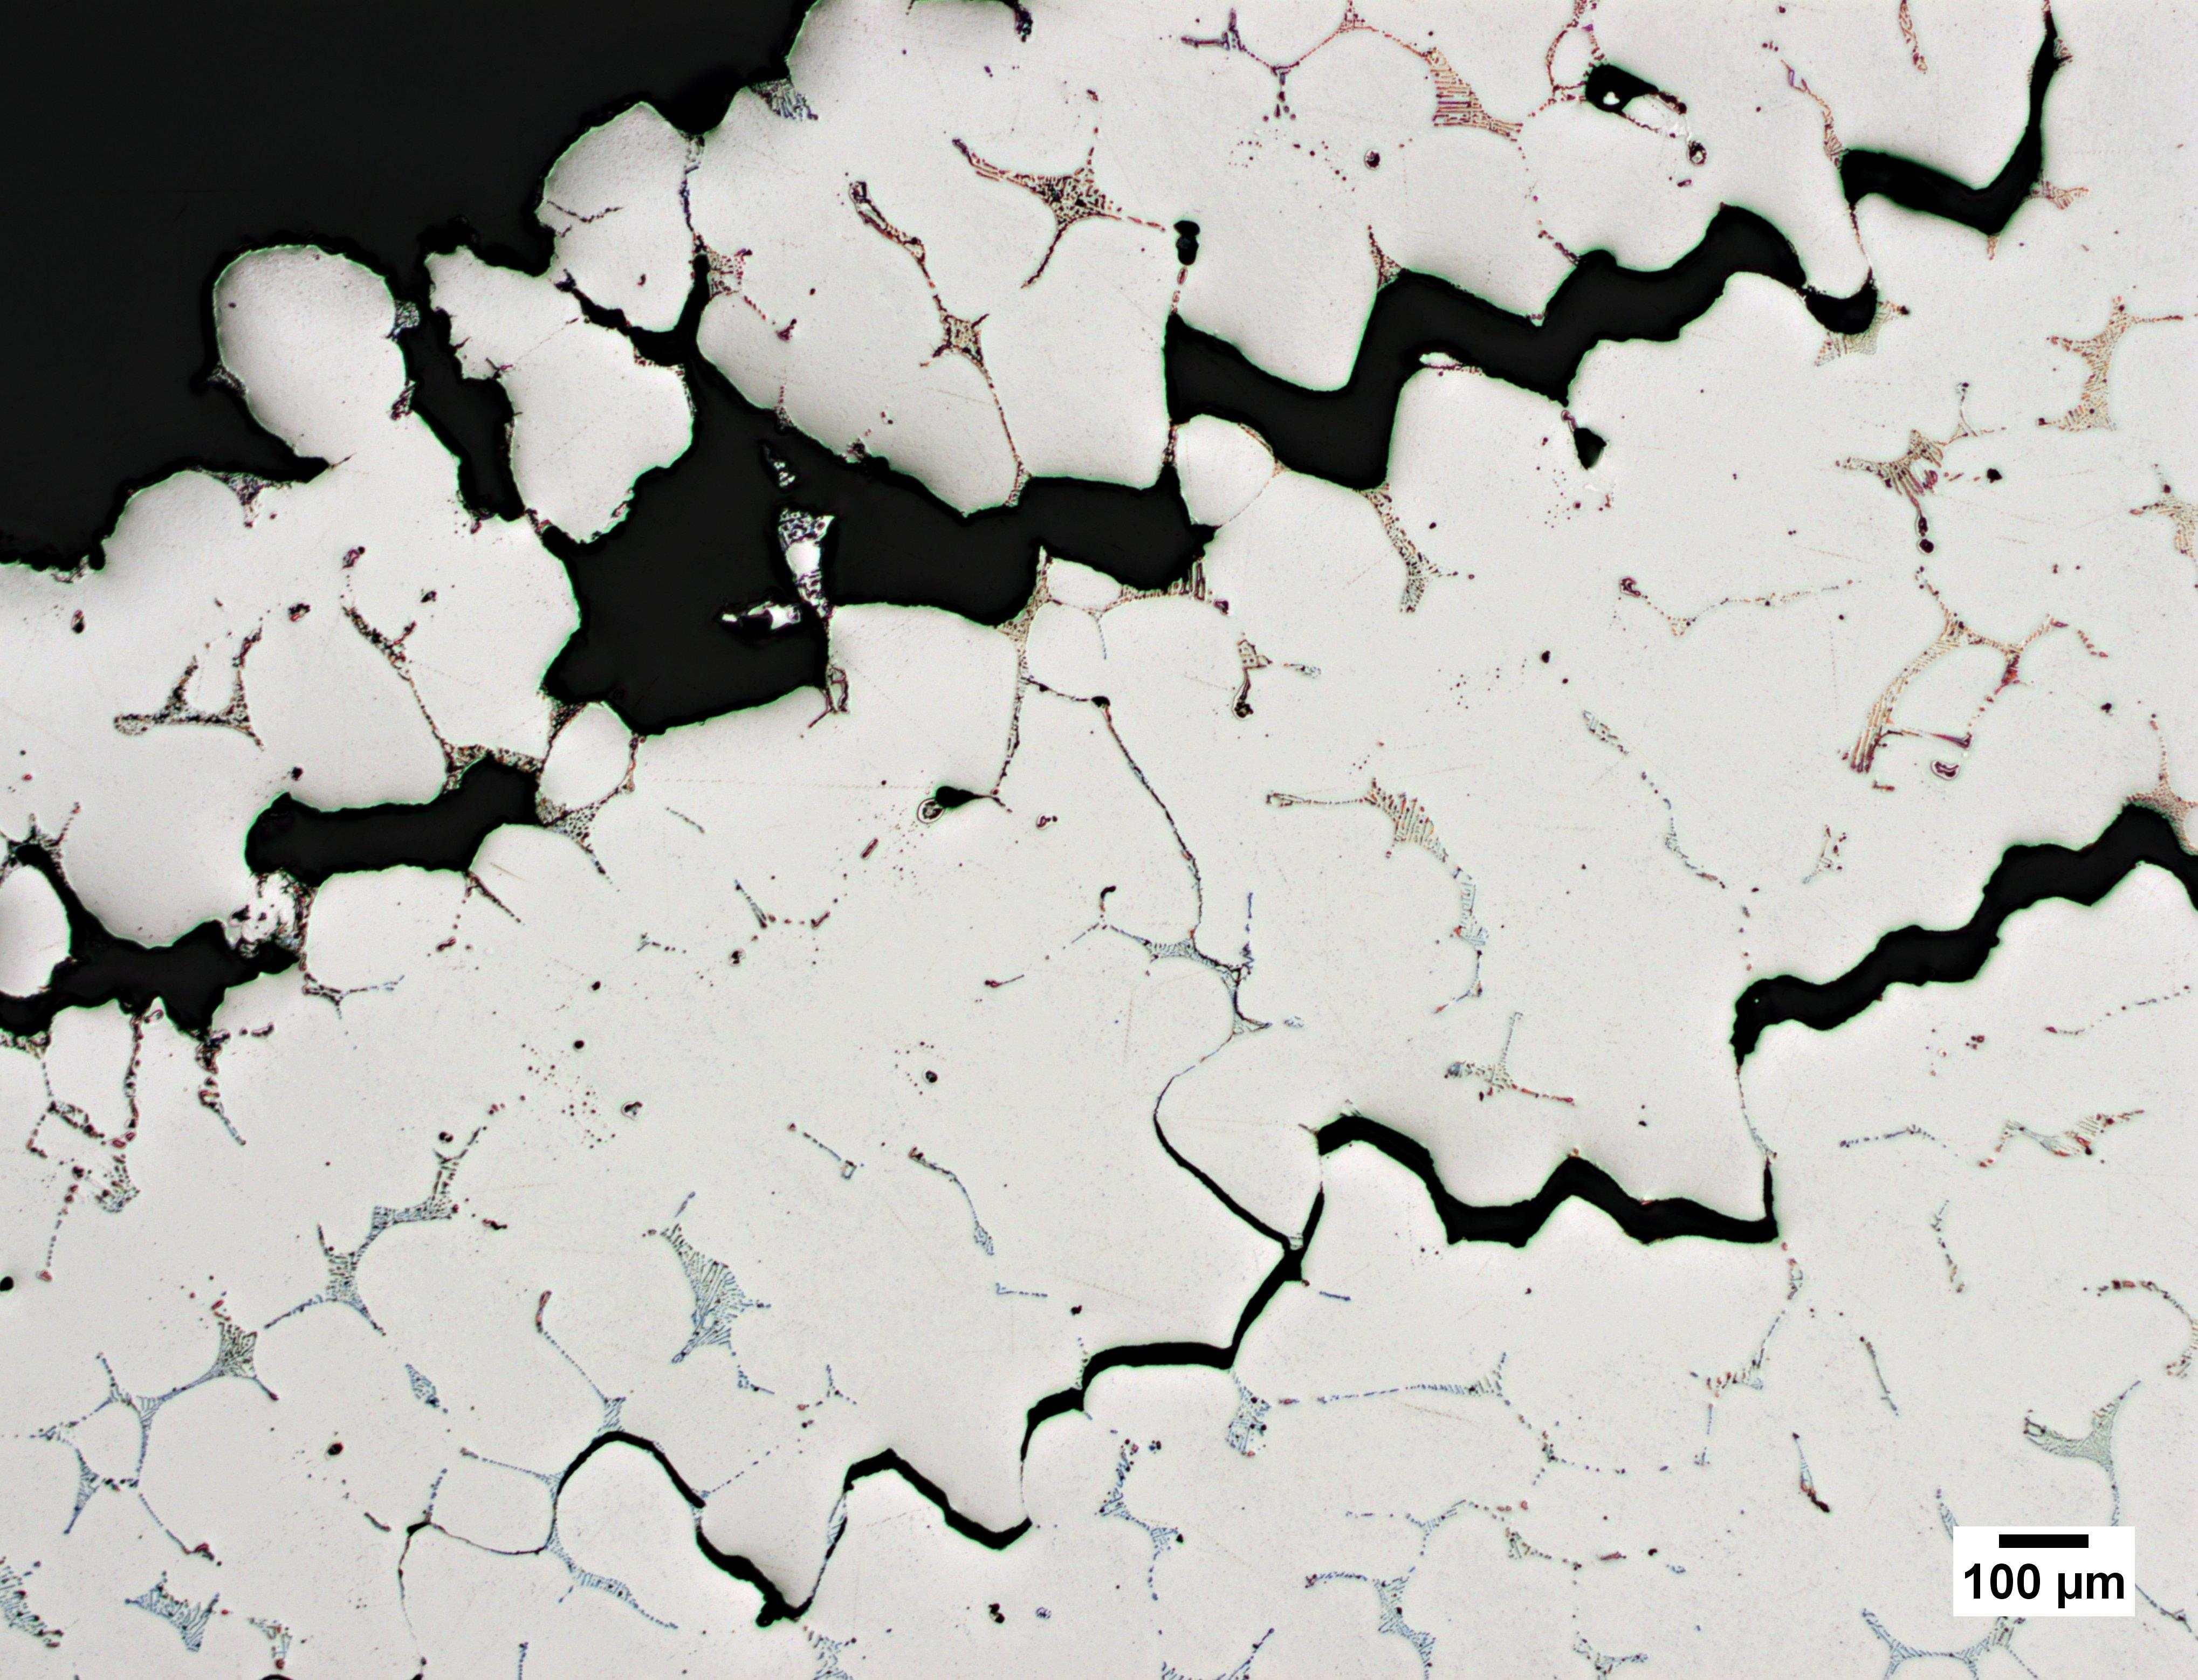
\includegraphics[width=4.7in]{figures/metallography/c5-oh-2375-50x}}\\
% \subfloat[200X]{\label{subfig:c5-oh-2375-200X}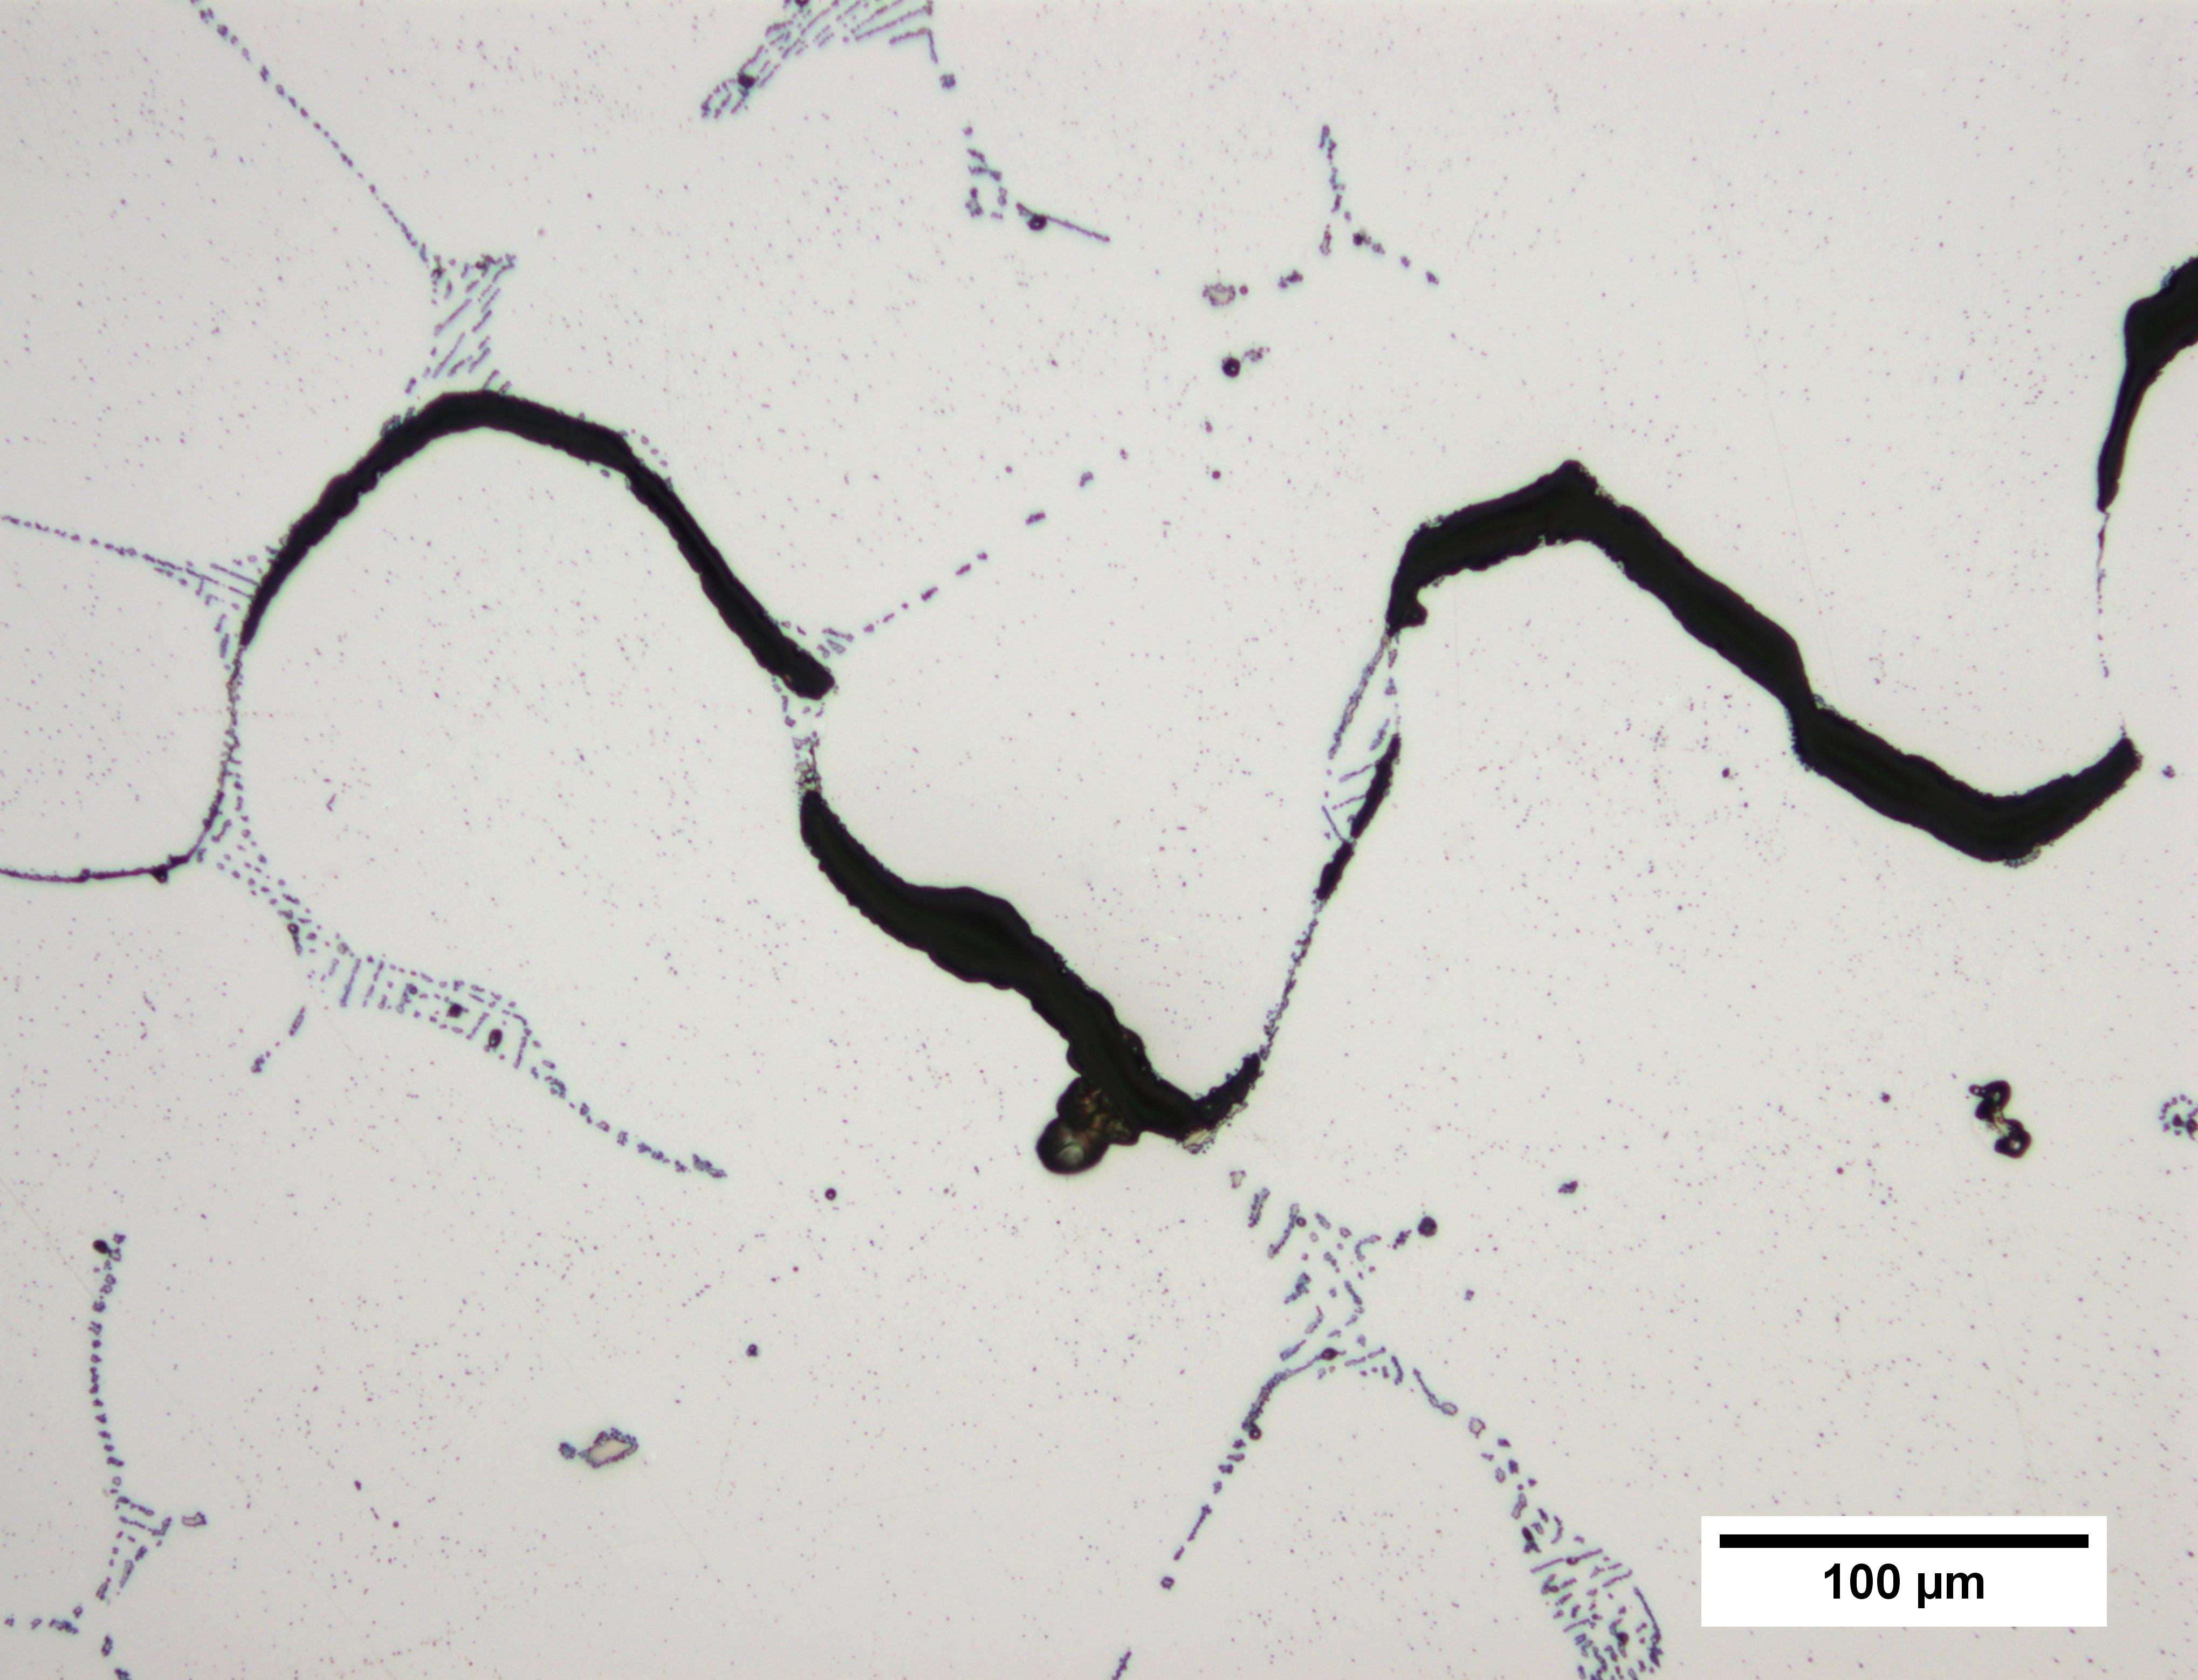
\includegraphics[width=4.7in]{figures/metallography/c5-oh-2375-200x}}

% \caption[Optical Micrographs Showing the Fracture Path as Revealed in a Longitudinal Section Through the Cone~5 2375\textdegree{}F On-Heating Hot Ductility Sample.]{Optical Micrographs Showing the Fracture Path as Revealed in a Longitudinal Section Through the Cone~5 2375\textdegree{}F On-Heating (\gls{zdt}) Hot Ductility Sample, at (A) 50X (B) 200X, (C) 500X and (D) 1000X.  Etch: 10\% Oxalic Acid, Electrolytic.}
% \label{fig:c5-oh-2375}
% \end{figure}


% \begin{figure}
% \ContinuedFloat
% \centering
% \subfloat[500X]{\label{subfig:c5-oh-2375-500X}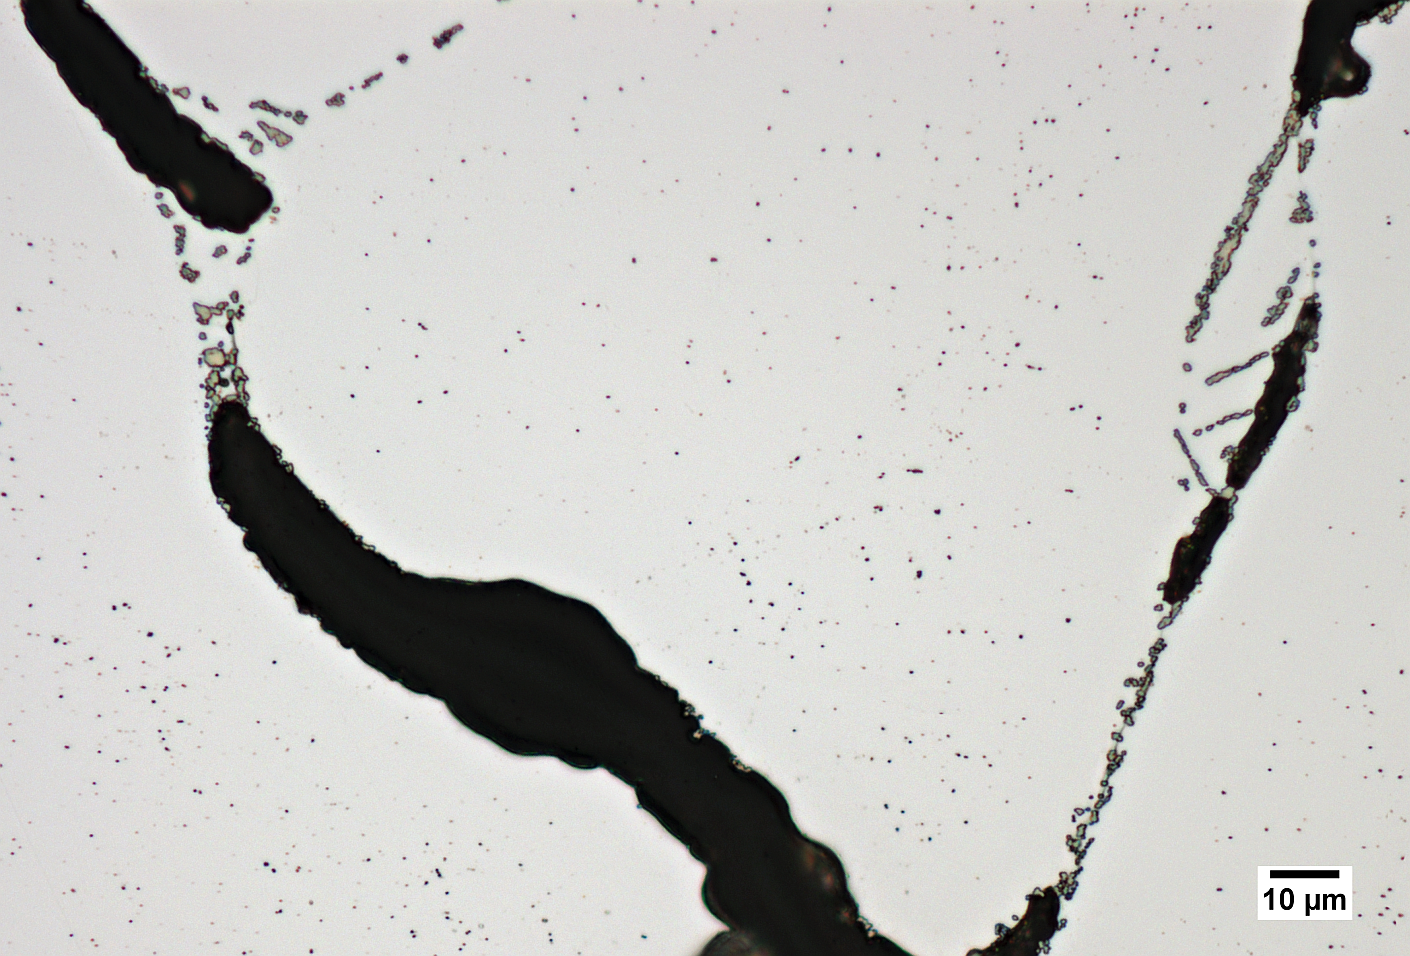
\includegraphics[width=4.7in]{figures/metallography/c5-oh-2375-500x}}

% \subfloat[1000X]{\label{subfig:c5-oh-2375-1000X}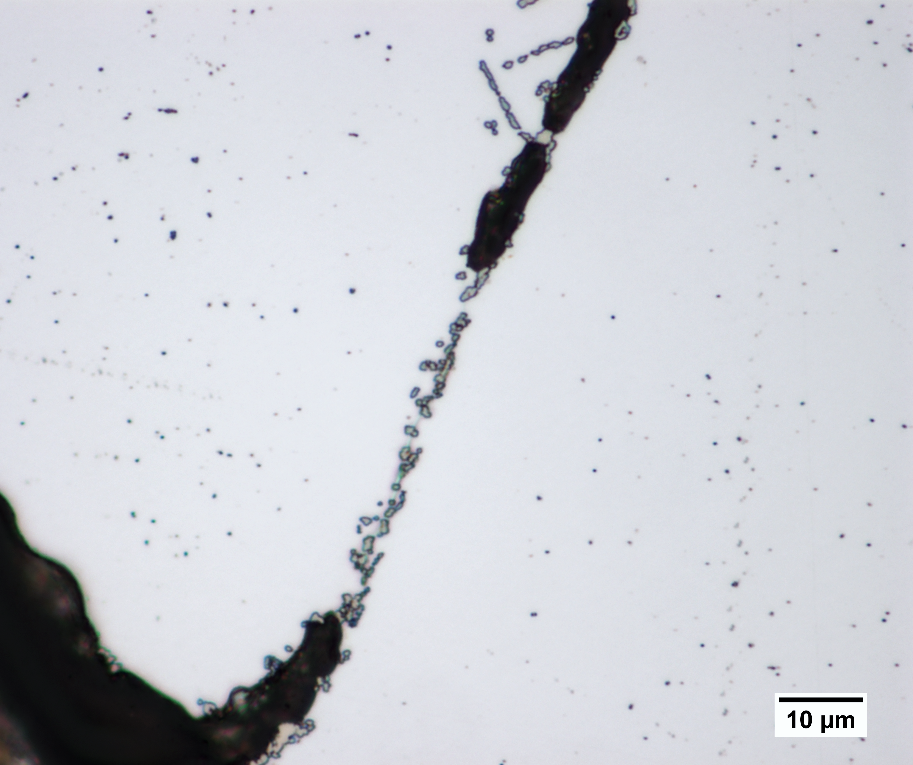
\includegraphics[width=4.7in]{figures/metallography/c5-oh-2375-1kx}}
% \caption[Optical Micrographs Showing the Fracture Path as Revealed in a Longitudinal Section Through the Cone~5 2375\textdegree{}F On-Heating Hot Ductility Sample.]{Optical Micrographs Showing the Fracture Path as Revealed in a Longitudinal Section Through the Cone~5 2375\textdegree{}F On-Heating (\gls{zdt}) Hot Ductility Sample, at (A) 50X (B) 200X, (C) 500X and (D) 1000X.  Etch: 10\% Oxalic Acid, Electrolytic.}

% \end{figure}


% \begin{figure}
% \centering
% \subfloat[200X]{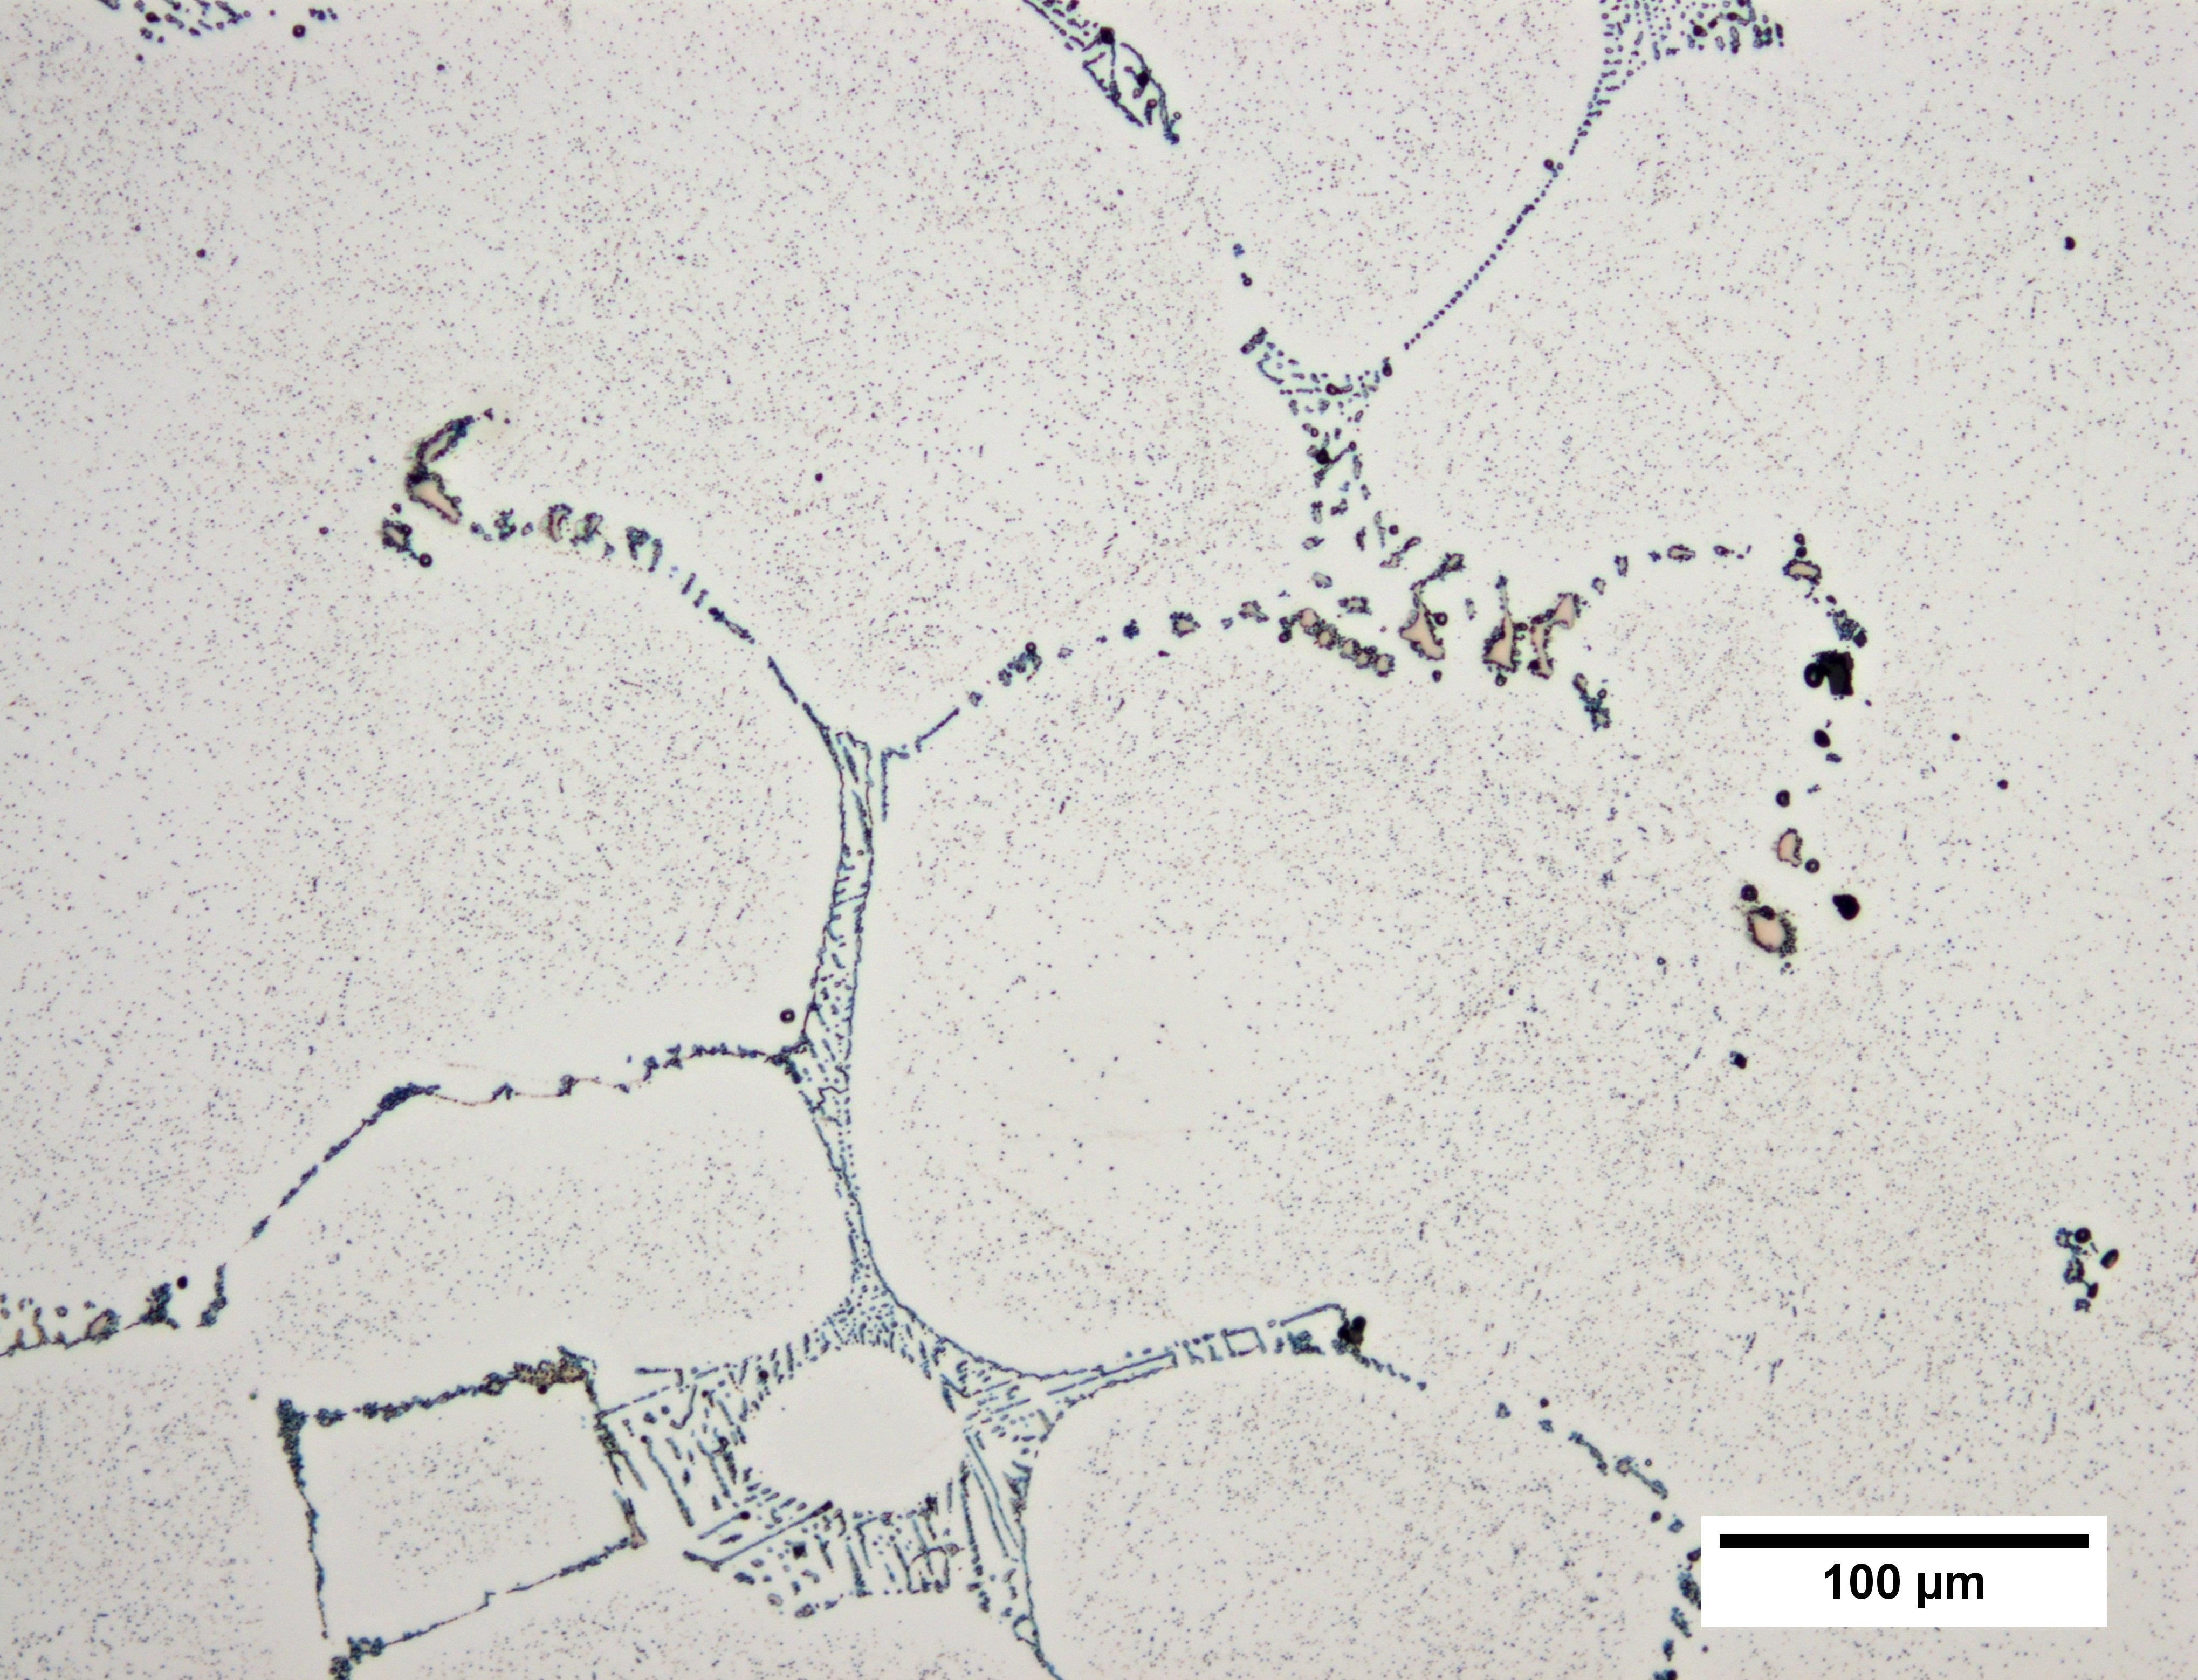
\includegraphics[width=4.7in]{figures/metallography/c5-oh-2375-remote-200x}}

% \subfloat[500X]{\label{subfig:c5-oh-2375-remote-500x}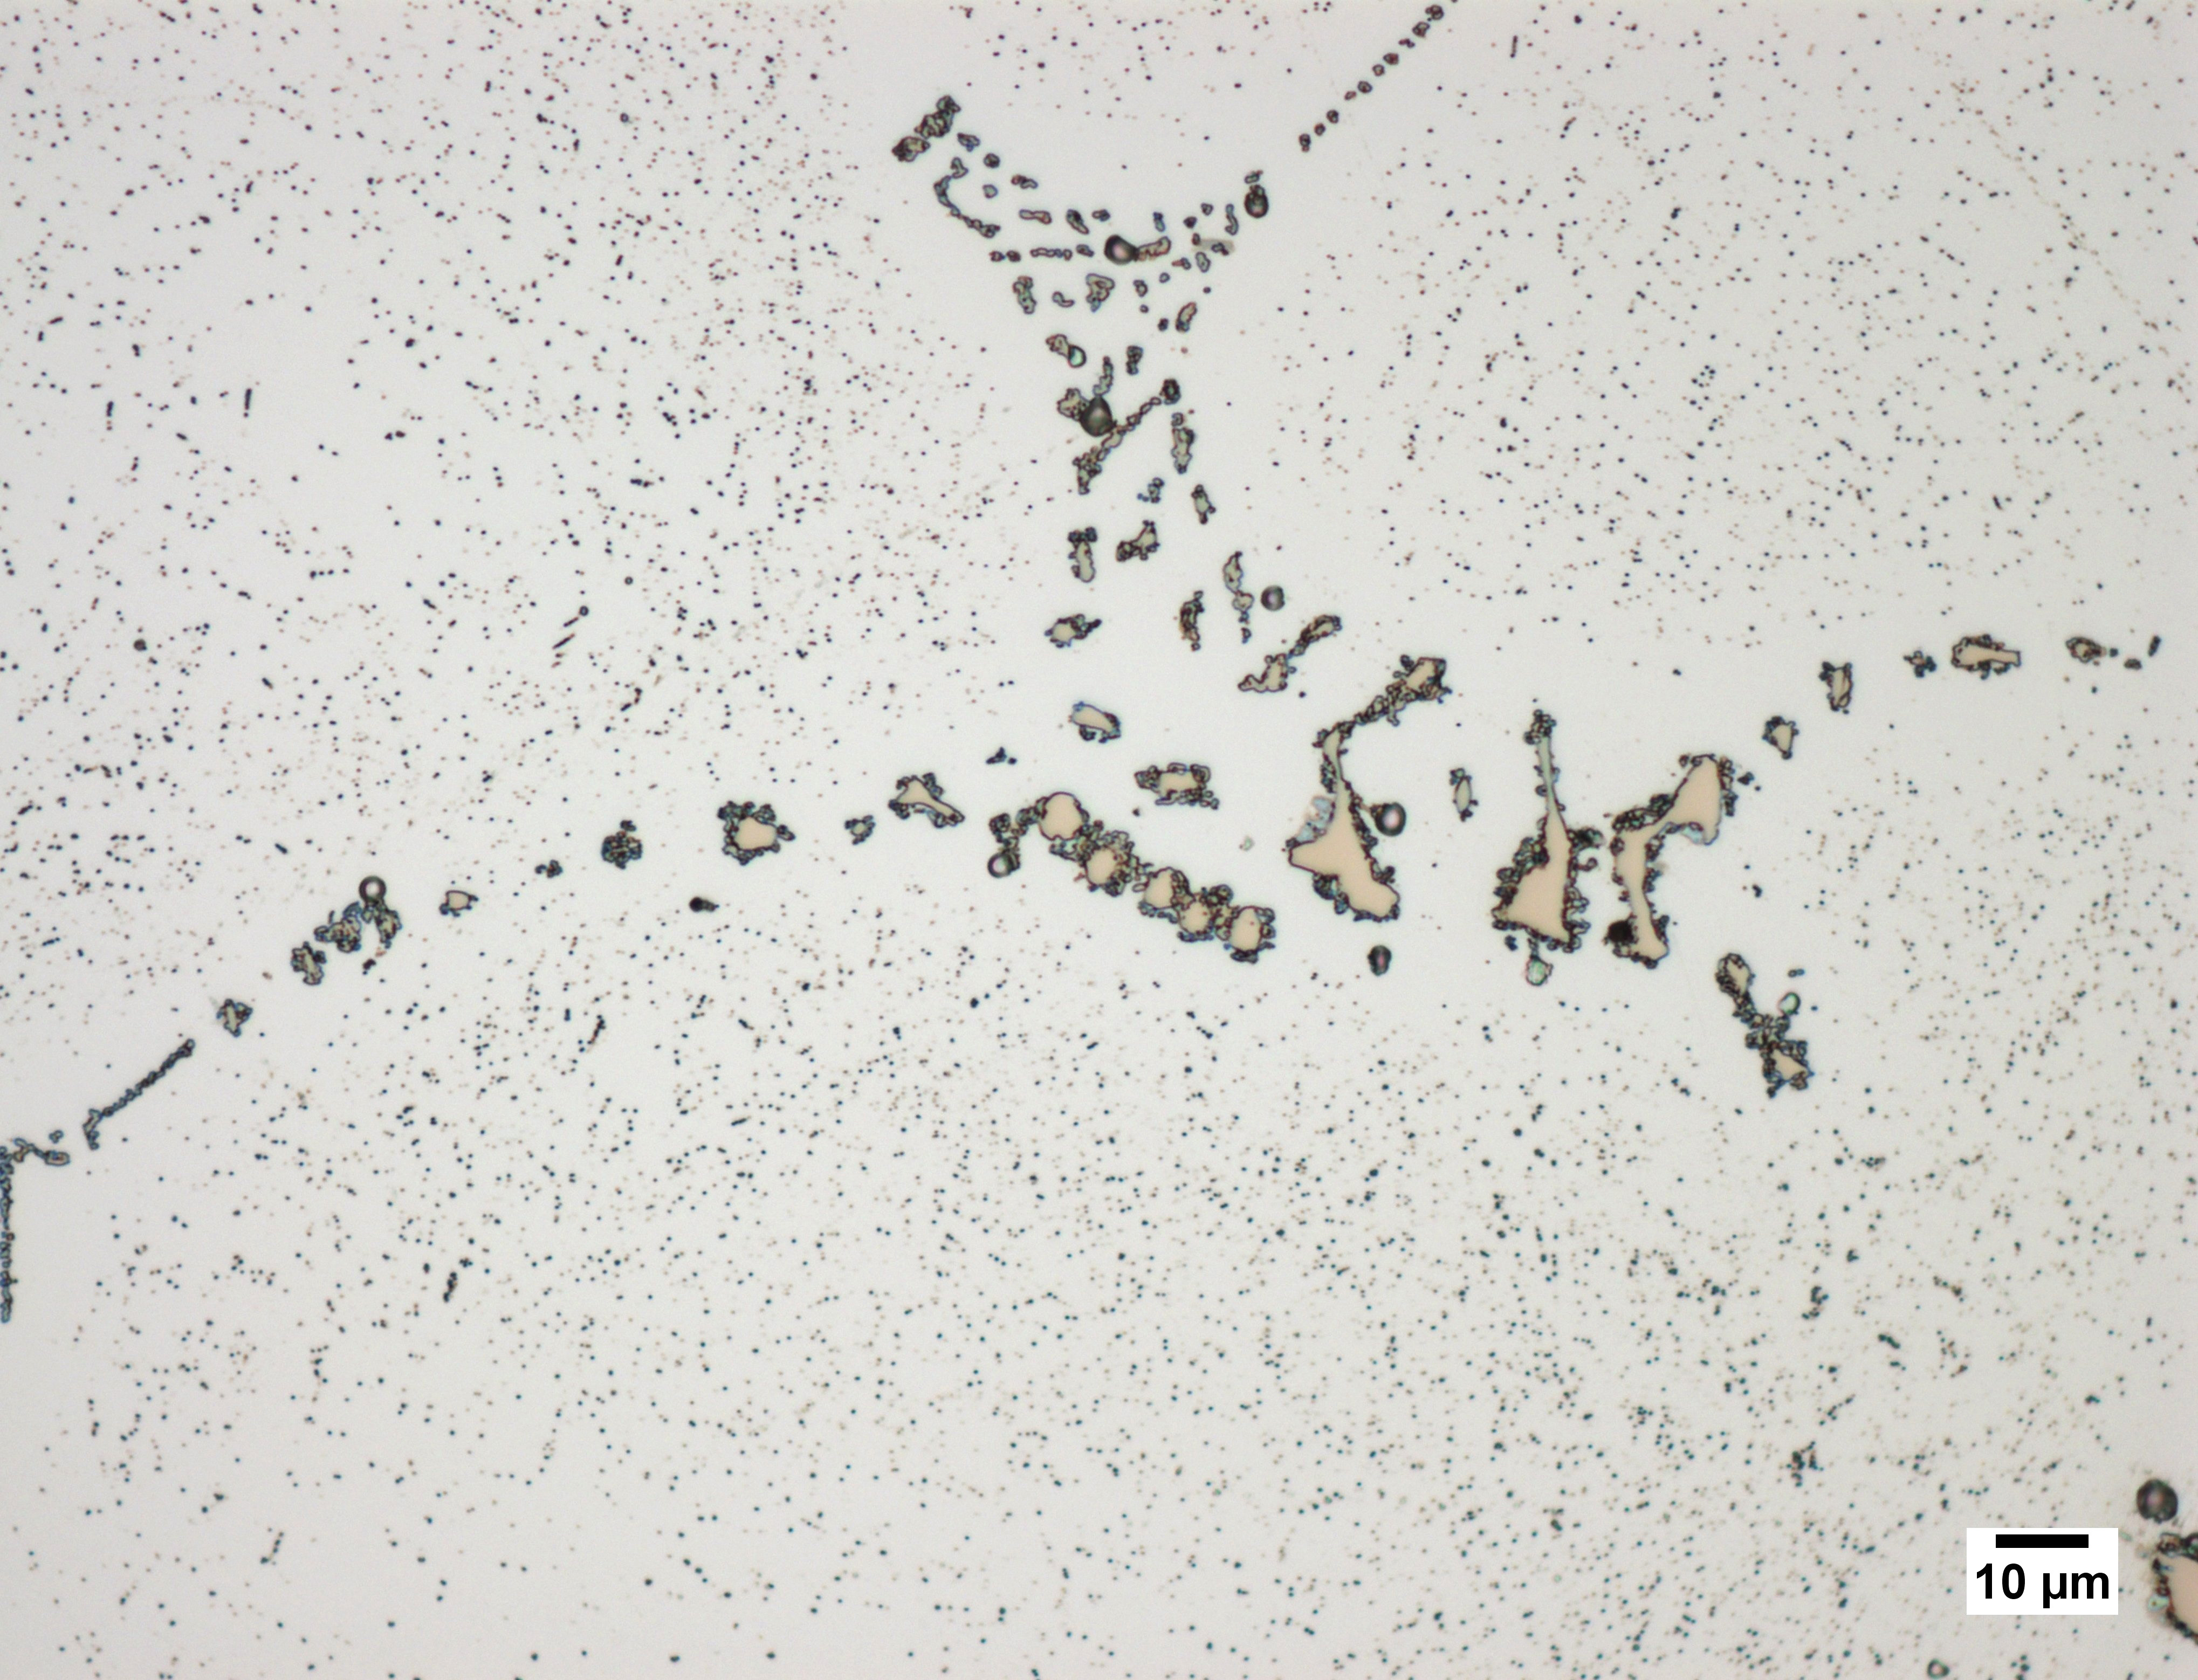
\includegraphics[width=4.7in]{figures/metallography/c5-oh-2375-remote-500x}}

% \caption{Optical Micrographs Showing the Microstructure of Unaffected Base Metal (Remote from the Fracture Location) in the Cone~5 2375\textdegree{}F On-Heating (\gls{zdt}) Hot Ductility Sample at (A) 200X and (B) 500X.  Etch: 10\% Oxalic Acid, Electrolytic.}
% \label{fig:c5-oh-2375-remote}
% \end{figure}



% Previous investigations (Hoffman and Colwell 1998; Hoffman and Gapinski 2001) of service-exposed 20Cr-32Ni-1Nb material with similar time in service indicated that the larger interdendritic phases were primarily niobium carbides (NbC), some of which were surrounded by a phase rich in Ni, Nb, and Si, while the intradendritic precipitates were determined to be mainly chromium carbides which precipitated as a result of service exposure.  The previously noted similarities in the hot ductility behavior are explained in light of the similarity of the as-received microstructures of the Cone~1 (``service-exposed'') and Cone~5 (``solution-annealed'') materials.  However, this was not the expected result based on the nominally reported material conditions since an earlier study on the repair weldability of 20Cr-32Ni-1Nb by Shi et al. (Shi, Lippold, and Ramirez 2010) indicated that solution annealed material showed a significantly different hot ductility response in terms of both on-heating and on-cooling behavior as compared to service-exposed material.  Therefore, the similar as-received microstructures of both Cone~1 and Cone~5, and the consequent similarities observed in the hot ductility characteristics, suggests that the weld joint region of Cone~5 (where the samples were extracted) was either not subjected to a solution annealing heat treatment or the parameters (temperature/time) were not adequate for an effective solution anneal, contrary to the information provided at the outset of this investigation.


% Regarding the Cone~5 On-Heating 2375\textdegree{}F (ZDT) hot ductility sample, examination of Figure 10a indicates that regions near the fracture surface showed a noticeably reduced extent of matrix precipitates compared a region remote from the fracture surface  (Figure 11).  This reduction is due to the dissolution of precipitates as a result of the high temperature exposure from the simulated thermal cycle.  It is also apparent from Figure 10a that the crack paths proceed along the interdendritic boundaries; Figure 10c and Figure 10d show that the crack faces appear to be associated with the interdendritic secondary phases.  Cracking proceeds along these boundaries because they are the regions corresponding to the greatest degree of solute segregation and resulting formation of low-melting point constituents; consequently, melting will begin at these regions first during the high temperatures imposed during the simulated thermal cycle of the hot ductility test.  The identity of the interdendritic phases has not yet been verified but this will be pursued as part of the future work.

\subsection{On-Cooling Hot Ductility Tests}
\subsubsection{Cone~1 On-Cooling}
The near-surface region of the Cone~1 On-Cooling 2300F (C1 OC-2300) hot ductility sample is shown in Figure D. As with the C1 OH-2375 test (Figure ??), cracking is readily apparent with the crack paths following the interdendritic boundaries, and a significant fraction of the intradendritic precipitates have dissolved. However, compared with C1 OH-2375, the C1 OC-2300 sample exhibits a much larger extent of liquid formation near the fracture surface, which is apparent in Figure D and also at higher magnification in Figure E (see arrows). In these micrographs the liquid films are nearly continuous across the fracture surface. The greater extent of liquid is due to the longer duration of elevated temperature exposure for this sample, even though C1 OH-2375 and C1 OC-2300 experienced the same peak temperature (recall that the peak temperature for the on-cooling tests was chosen as the on-heating \gls{zdt}, equal to 2375\textdegree{}F). In the on-cooling tests, the sample spends a definite amount of time () near the peak of the welding thermal cycle before being fractured on-cooling; in comparison, the on-heating \gls{zdt} sample (C1 OH-2375) was fractured immediately upon reaching the peak temperature with correspondingly less time for liquid formation.

Figure F presents a higher magnification view of the region near the tip of the crack shown in Figure D. Extensive formerly-melted regions are apparent around the interdendritic phases and along the crack faces. The crack tip region in Figure F is shown in the SEM micrographs in Figure G, with the corresponding EDS analysis results (from the box in Figure Gb) given in Figure H. There are numerous small particles located on the crack faces and on the interdendritic boundary ahead of the crack tip, which are enriched in Nb (Figure H); the Fe, Cr, and Ni peaks most likely originate from the surrounding matrix. Notably, Si enrichment above the nominal alloy composition is not observed which suggests the Ni-Nb-Si silicide phase is not present in the interdendritic region. 

The formerly melted region surrounding some of the interdendritic phases in Figure D is evaluated further in the SEM micrographs in Figure I with corresponding EDS spot analysis results in Figure J. The quantitative EDS results indicate that the liquid surrounding the interdendritic phases is essentially similar to the nominal alloy composition and is not enriched in Ni, Nb, or Si. This fact suggests that the formation of liquid in this region (along the interdendritic boundaries) is not due to melting of Ni-Nb-Si phases during the simulated on-cooling thermal cycle.

%C1 On-cooling figures
\begin{figure}
\centering
\subfloat[1000X]{\label{subfig:c1-oc-2300-sem-liquid-1kx}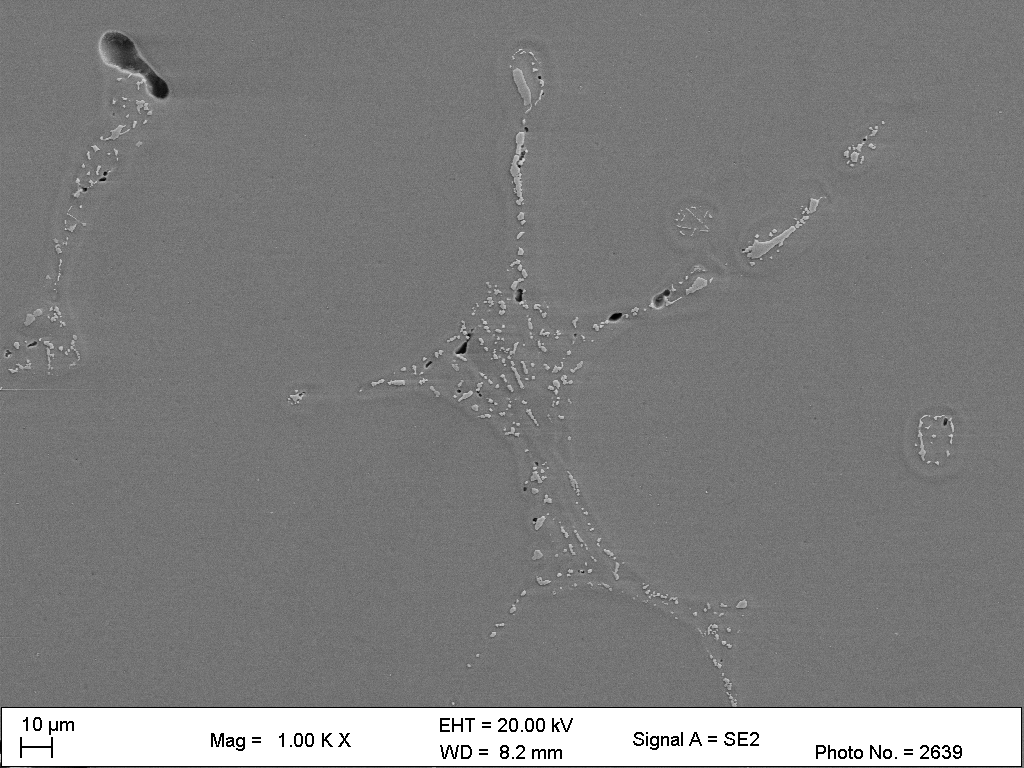
\includegraphics[width=4.7in]{figures/metallography/c1-oc-2300-liquid-L1-1kx-01.png}} \\
\subfloat[5000X]{\label{subfig:c1-oc-2300-sem-liquid-5kx}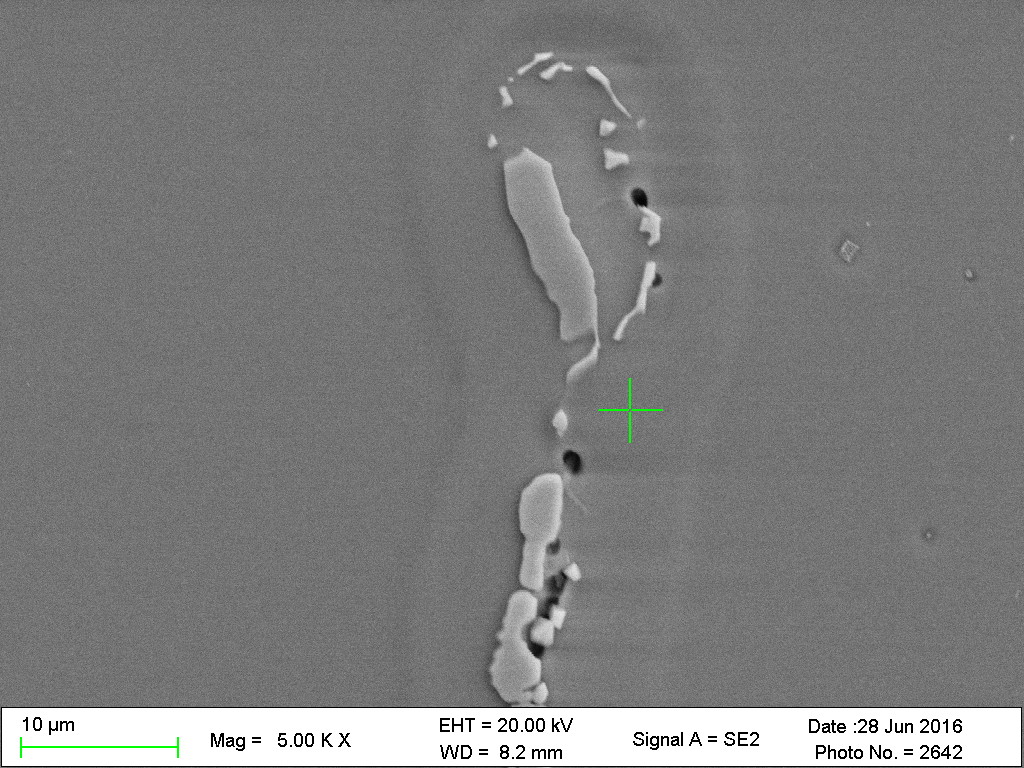
\includegraphics[width=4.7in]{figures/metallography/c1-oc-2300-liquid-L1-5kx-04.png}}
\caption[]{\Gls{sem} micrographs showing evidence of liquid film around interdendritic phases adjacent to the fracture surface in the Cone~1 On-Cooling 2300\textdegree{}F hot ductility sample. \Gls{eds} spot analysis results for the indicated point in (b) are given in Figure~\ref{fig:c1-oc-2300-liquid-eds}.}
\label{fig:c1-oc-2300-sem-liquid}
\end{figure}

% \begin{figure}
% \centering
% \subfloat[Spot Analysis ``A'']{\label{subfig:c1-ar-eds-a}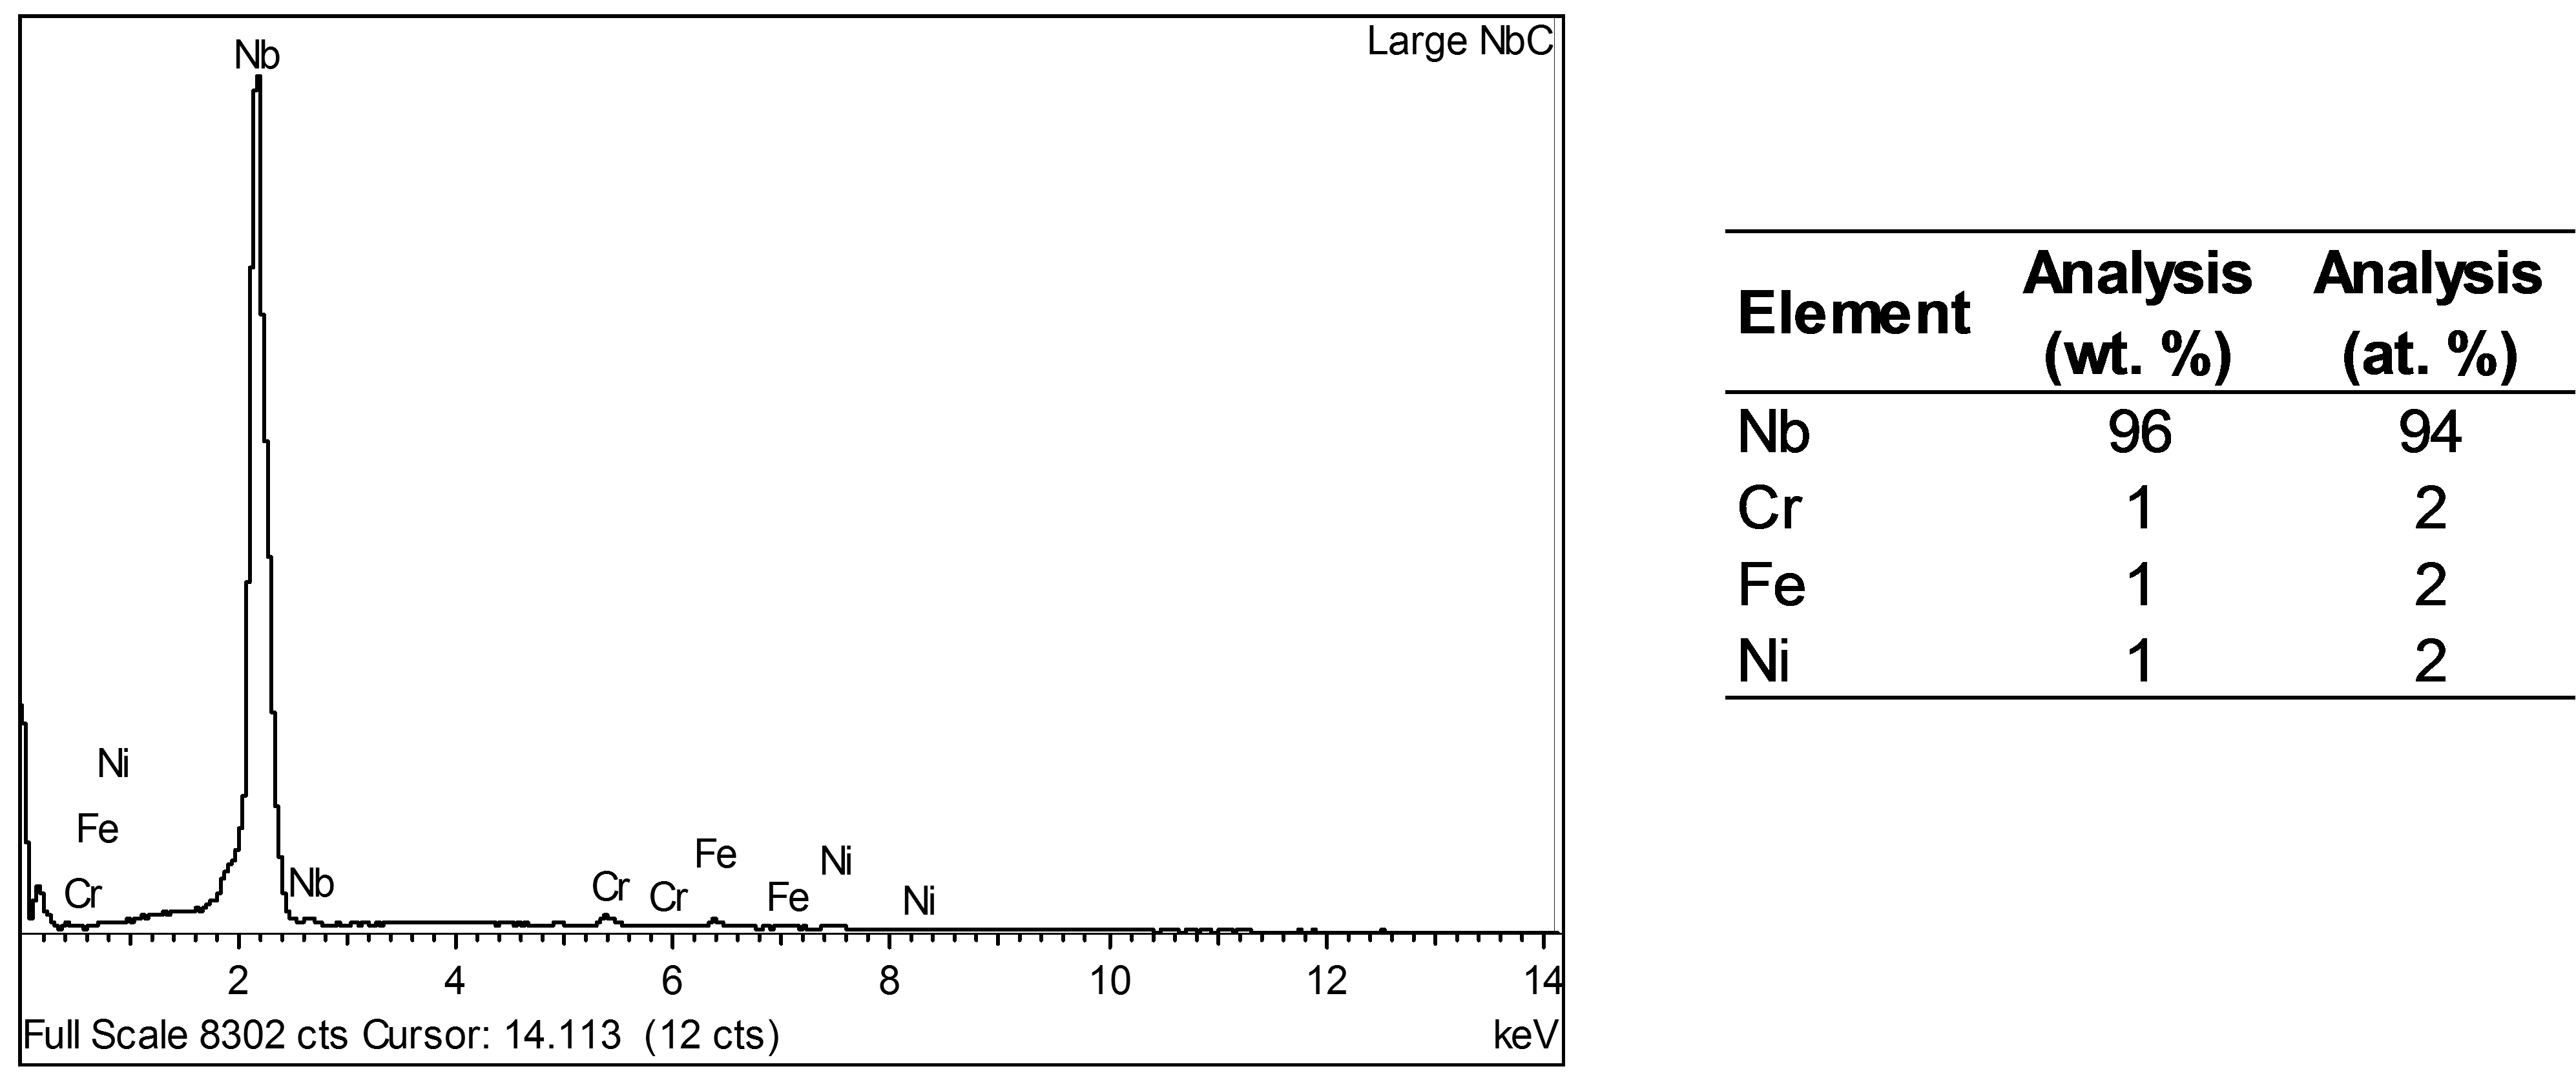
\includegraphics[width=4in]{figures/metallography/c1-ar-eds-table-L3-A.png}} \\
% \subfloat[Spot Analysis ``B'']{\label{subfig:c1-ar-eds-b}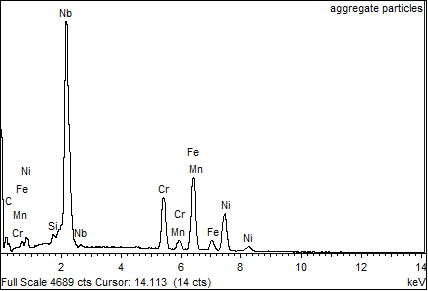
\includegraphics[width=4in]{figures/metallography/c1-ar-eds-L3-B.png}}
% \caption[]{\Gls{eds} spot analysis results for locations ``A'' and ``B'' identified in Figure~\ref{subfig:c1-ar-sem-5kx} for as-received Cone~1 material.}
% \label{fig:c1-oc-2300-liquid-eds}
% \end{figure}


\subsubsection{Cone~5 On-Cooling}